\setchapterstyle{kao}
\setchapterpreamble[u]{\margintoc}

\chapter{Monte Carlo Event Generation and Detector Simulation}
\labch{signal_simulation}

Like many analyses in IceCube, this work is based on MC simulations. The initial step for all particle (non-noise) simulation is the generation of events from selected initial distributions and fluxes. Events are the primary particle and all particles produced in the interaction with the ice. The particles are then propagated through the ice, producing Cherenkov photons, which are propagated further until they reach a DOM or are absorbed in the ice. If they hit a DOM the detector response is simulated. Splitting the simulation steps has the advantage of reusing the outputs of for example the generation step to propagate the particles with different ice model, in order to estimate the systematic impacts of uncertainties of the ice properties. A similar approach can be taken for varying detector response, before starting the event selection. Through this a more efficient (reduced) use of computing resources can be achieved.

The central part of this thesis is the HNL signal simulation itself. Since this is the first search for HNLs with IceCube DeepCore, there was no prior knowledge of the number of events expected per year nor of the performance in terms of reconstruction and classification accuracy. This chapter describes the first HNL event generation developed for IceCube DeepCore. Two avenues of generation were pursued in parallel. A collection of model-independent samples is explained in \refsec{model_independent_simulation}. They were used for performance benchmarking and for cross-checks to validate the physically accurate, model-dependent event generation, which is described in \refsec{model_specific_simulation}. The event generation for SM background events is briefly described in \refsec{sm_event_generation}, followed by the detector response simulation in \refsec{detector_simulation}. The detector response is identically applied to both signal and background events.


\section{Model-Independent Heavy Neutral Lepton Event Generation} \labsec{model_independent_simulation}

To investigate the potential of IceCube to detect HNLs by identifying the unique double cascade morphology explained in \refsec{double_cascade_morphology}, a model-independent double cascade generator was developed, where the kinematics of each cascade can be controlled directly. Using this generator, several simulation samples were produced to investigate the performance of IceCube DeepCore to detect low-energy double cascades, dependent on their properties. All samples are produced using a collection of custom generator functions \cite{cascade_generator_functions} that place two EM cascade vertices with variable energy and direction at configurable locations in the detector.


\subsection{Simplistic Samples} \labsec{simplistic_samples}

\todo{add/move event views to here? or draw a schematic of these events? (ORANGE)}

To investigate the best-case and the worst-case double cascade event scenarios, two samples are produced in the DeepCore volume: straight up-going events ($\cos(\theta)=-1$) that are centered on a string and horizontal events ($\cos(\theta)=0$). The first sample is used to investigate one of the most promising scenarios to detect a double cascade, where both cascade centers are located on a DeepCore string and the directions are directly up-going. One of the DeepCore strings was randomly chosen as the $x$-$y$ coordinate for this sample. As already mentioned in \refsec{deepcore}, DeepCore strings have higher quantum efficiency DOMs and a denser vertical spacing, making them better to detect low-energy events that produce little light. To produce the events, the $x,y$ position of the cascades is fixed to the center of the string while the $z$ positions are each sampled uniformly along the axis of the string. Note that this will therefore not produce a uniform length distribution between the cascades. The positions are defined in the IceCube coordinate system that was introduced in \refsec{icecube}. The energies are sampled uniformly between \SIrange[range-phrase={~and~}]{0.0}{60.0}{\gev}, to generously cover the region where $\nu_\mu\rightarrow\nu_\tau$ appearance is maximized. The time of the lower cascade is set to $t_0=\SI{0.0}{\nano\second}$ and for the upper one to $t_1=L/c$, assuming the HNL travels at the speed of light, $c$. \reffig{simplified_gen_distris} shows the resulting energy distributions and the decay length distribution, where it can be seen how the uniform cascade energies sum into a non-uniform total energy, and the decay length distribution is also non-uniform due to the uniform $z$ sampling of both cascades, which sets the distance between them.

\begin{figure*}[h]
    \centering
    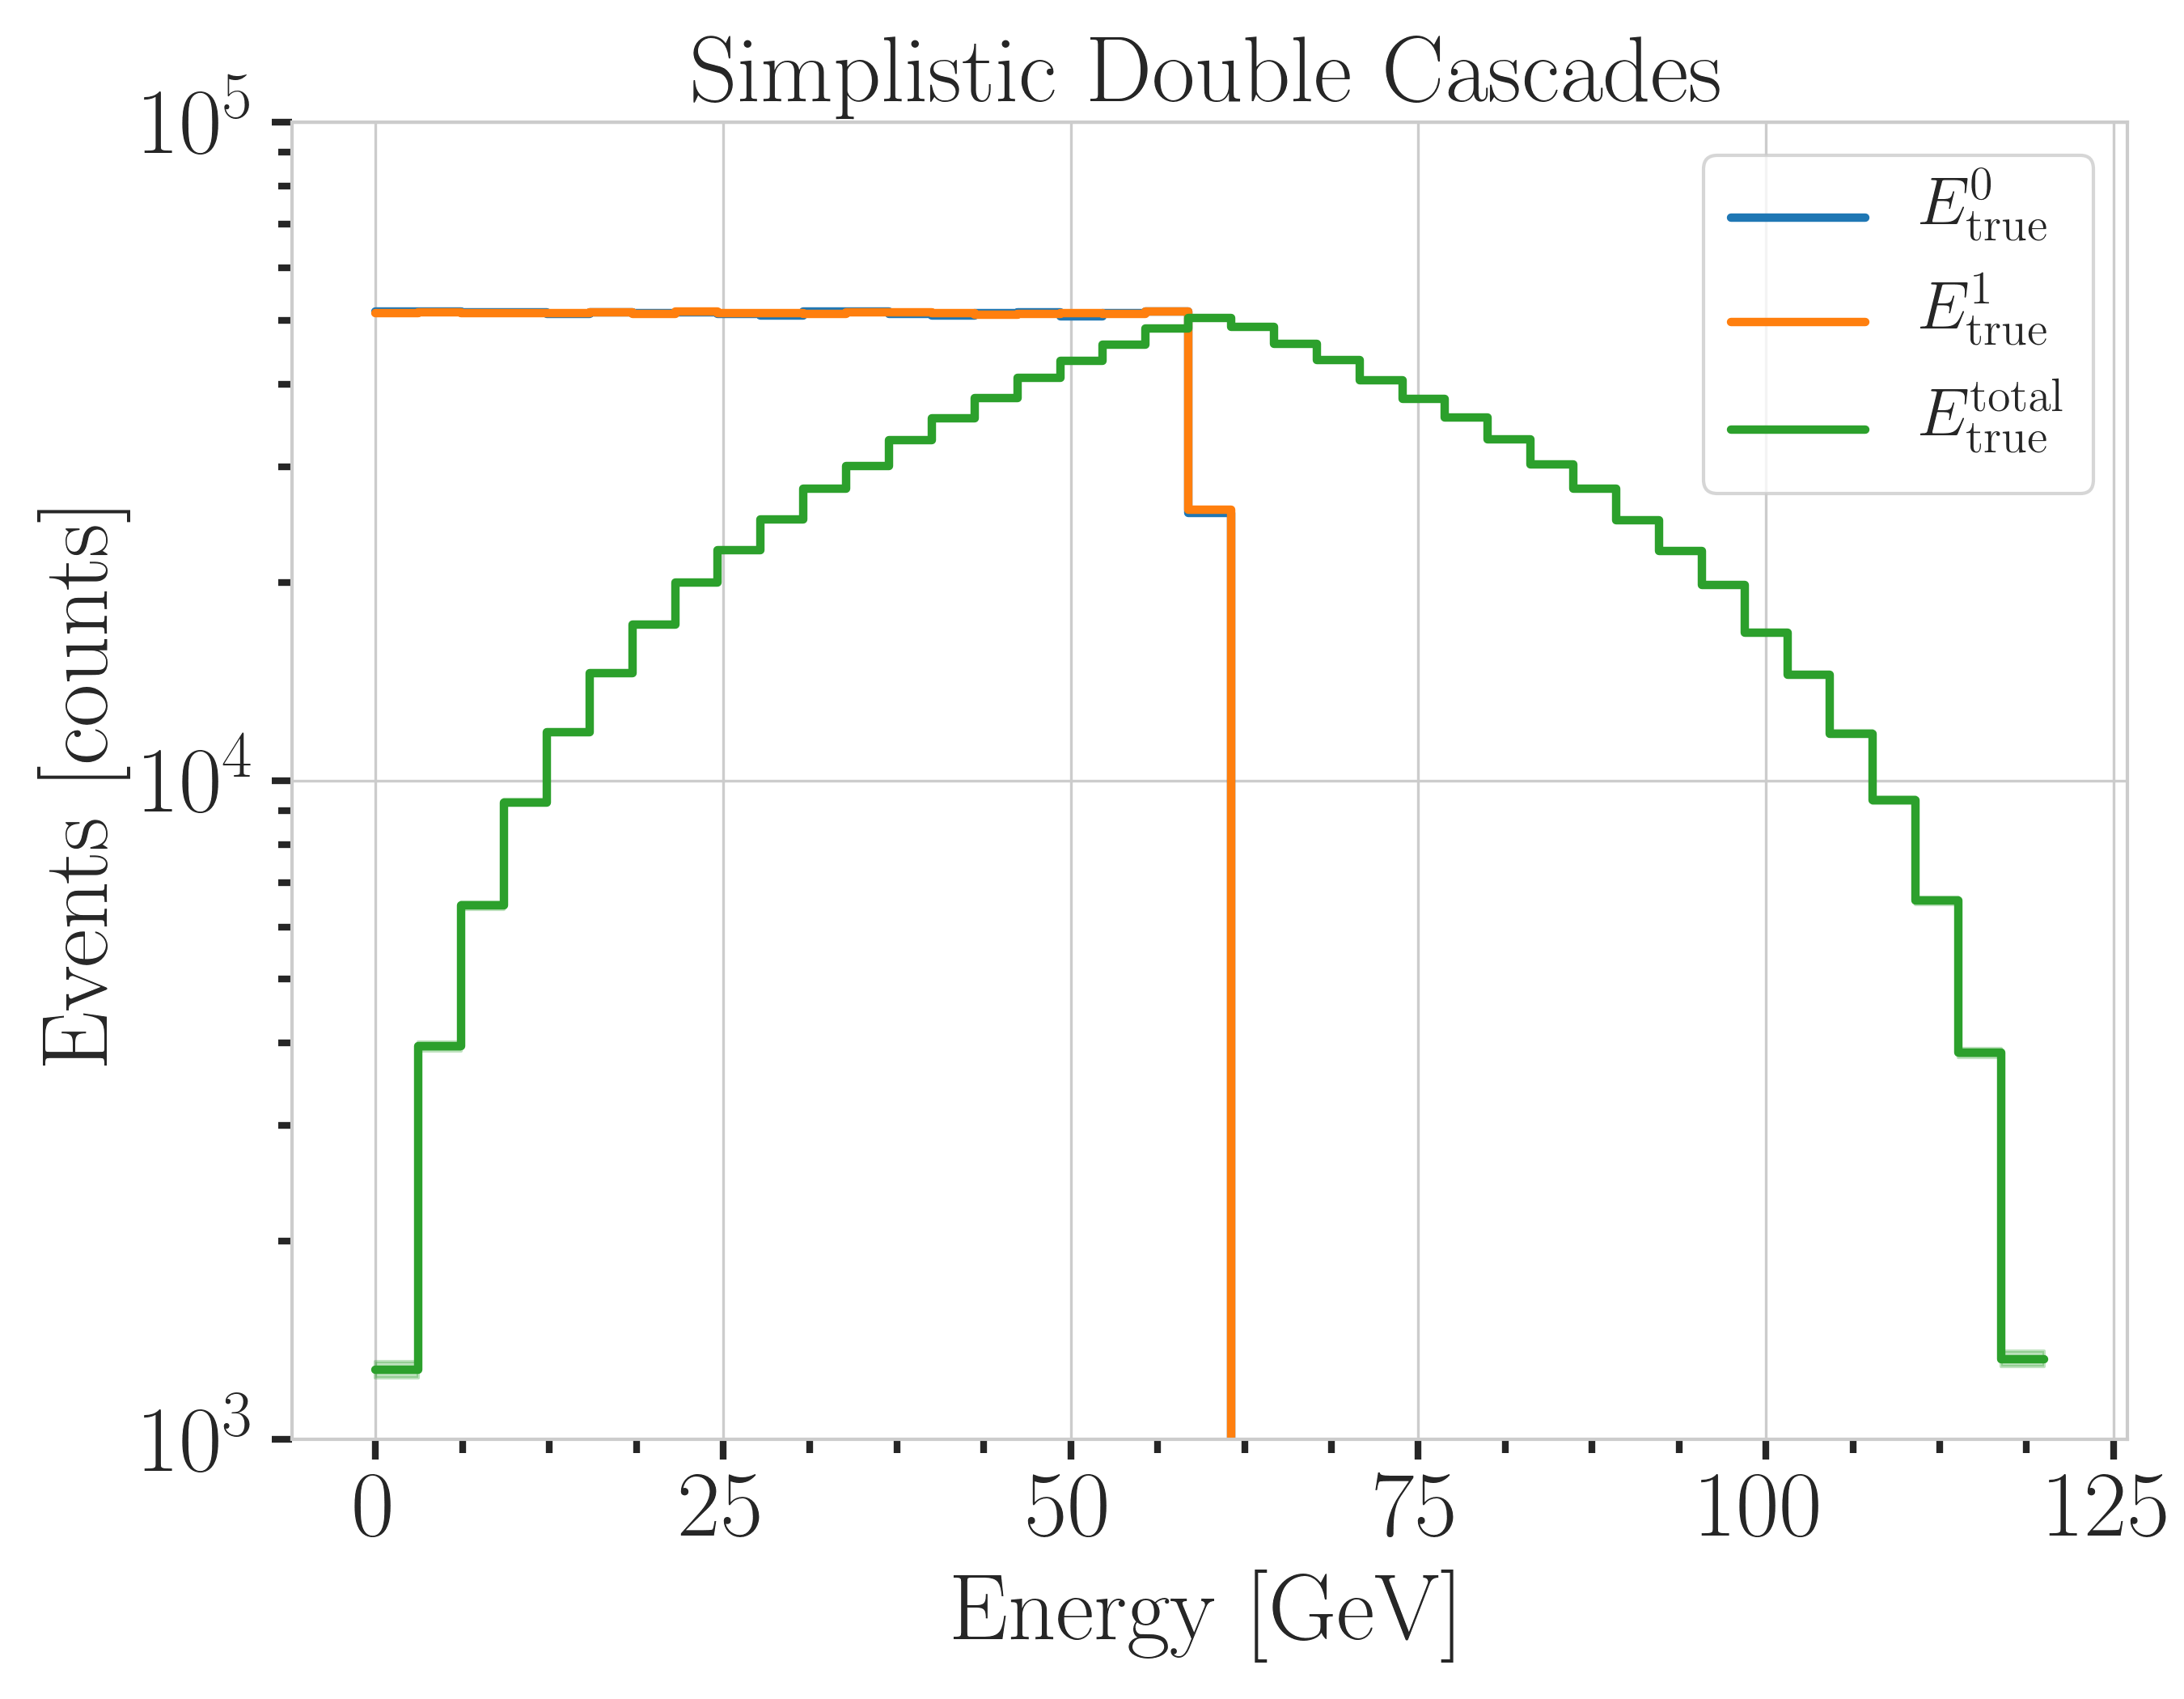
\includegraphics[width=.49\linewidth]{figures/model_independent_simulation/gen_level/simplistic_1_d_distr_all_energies.png}
    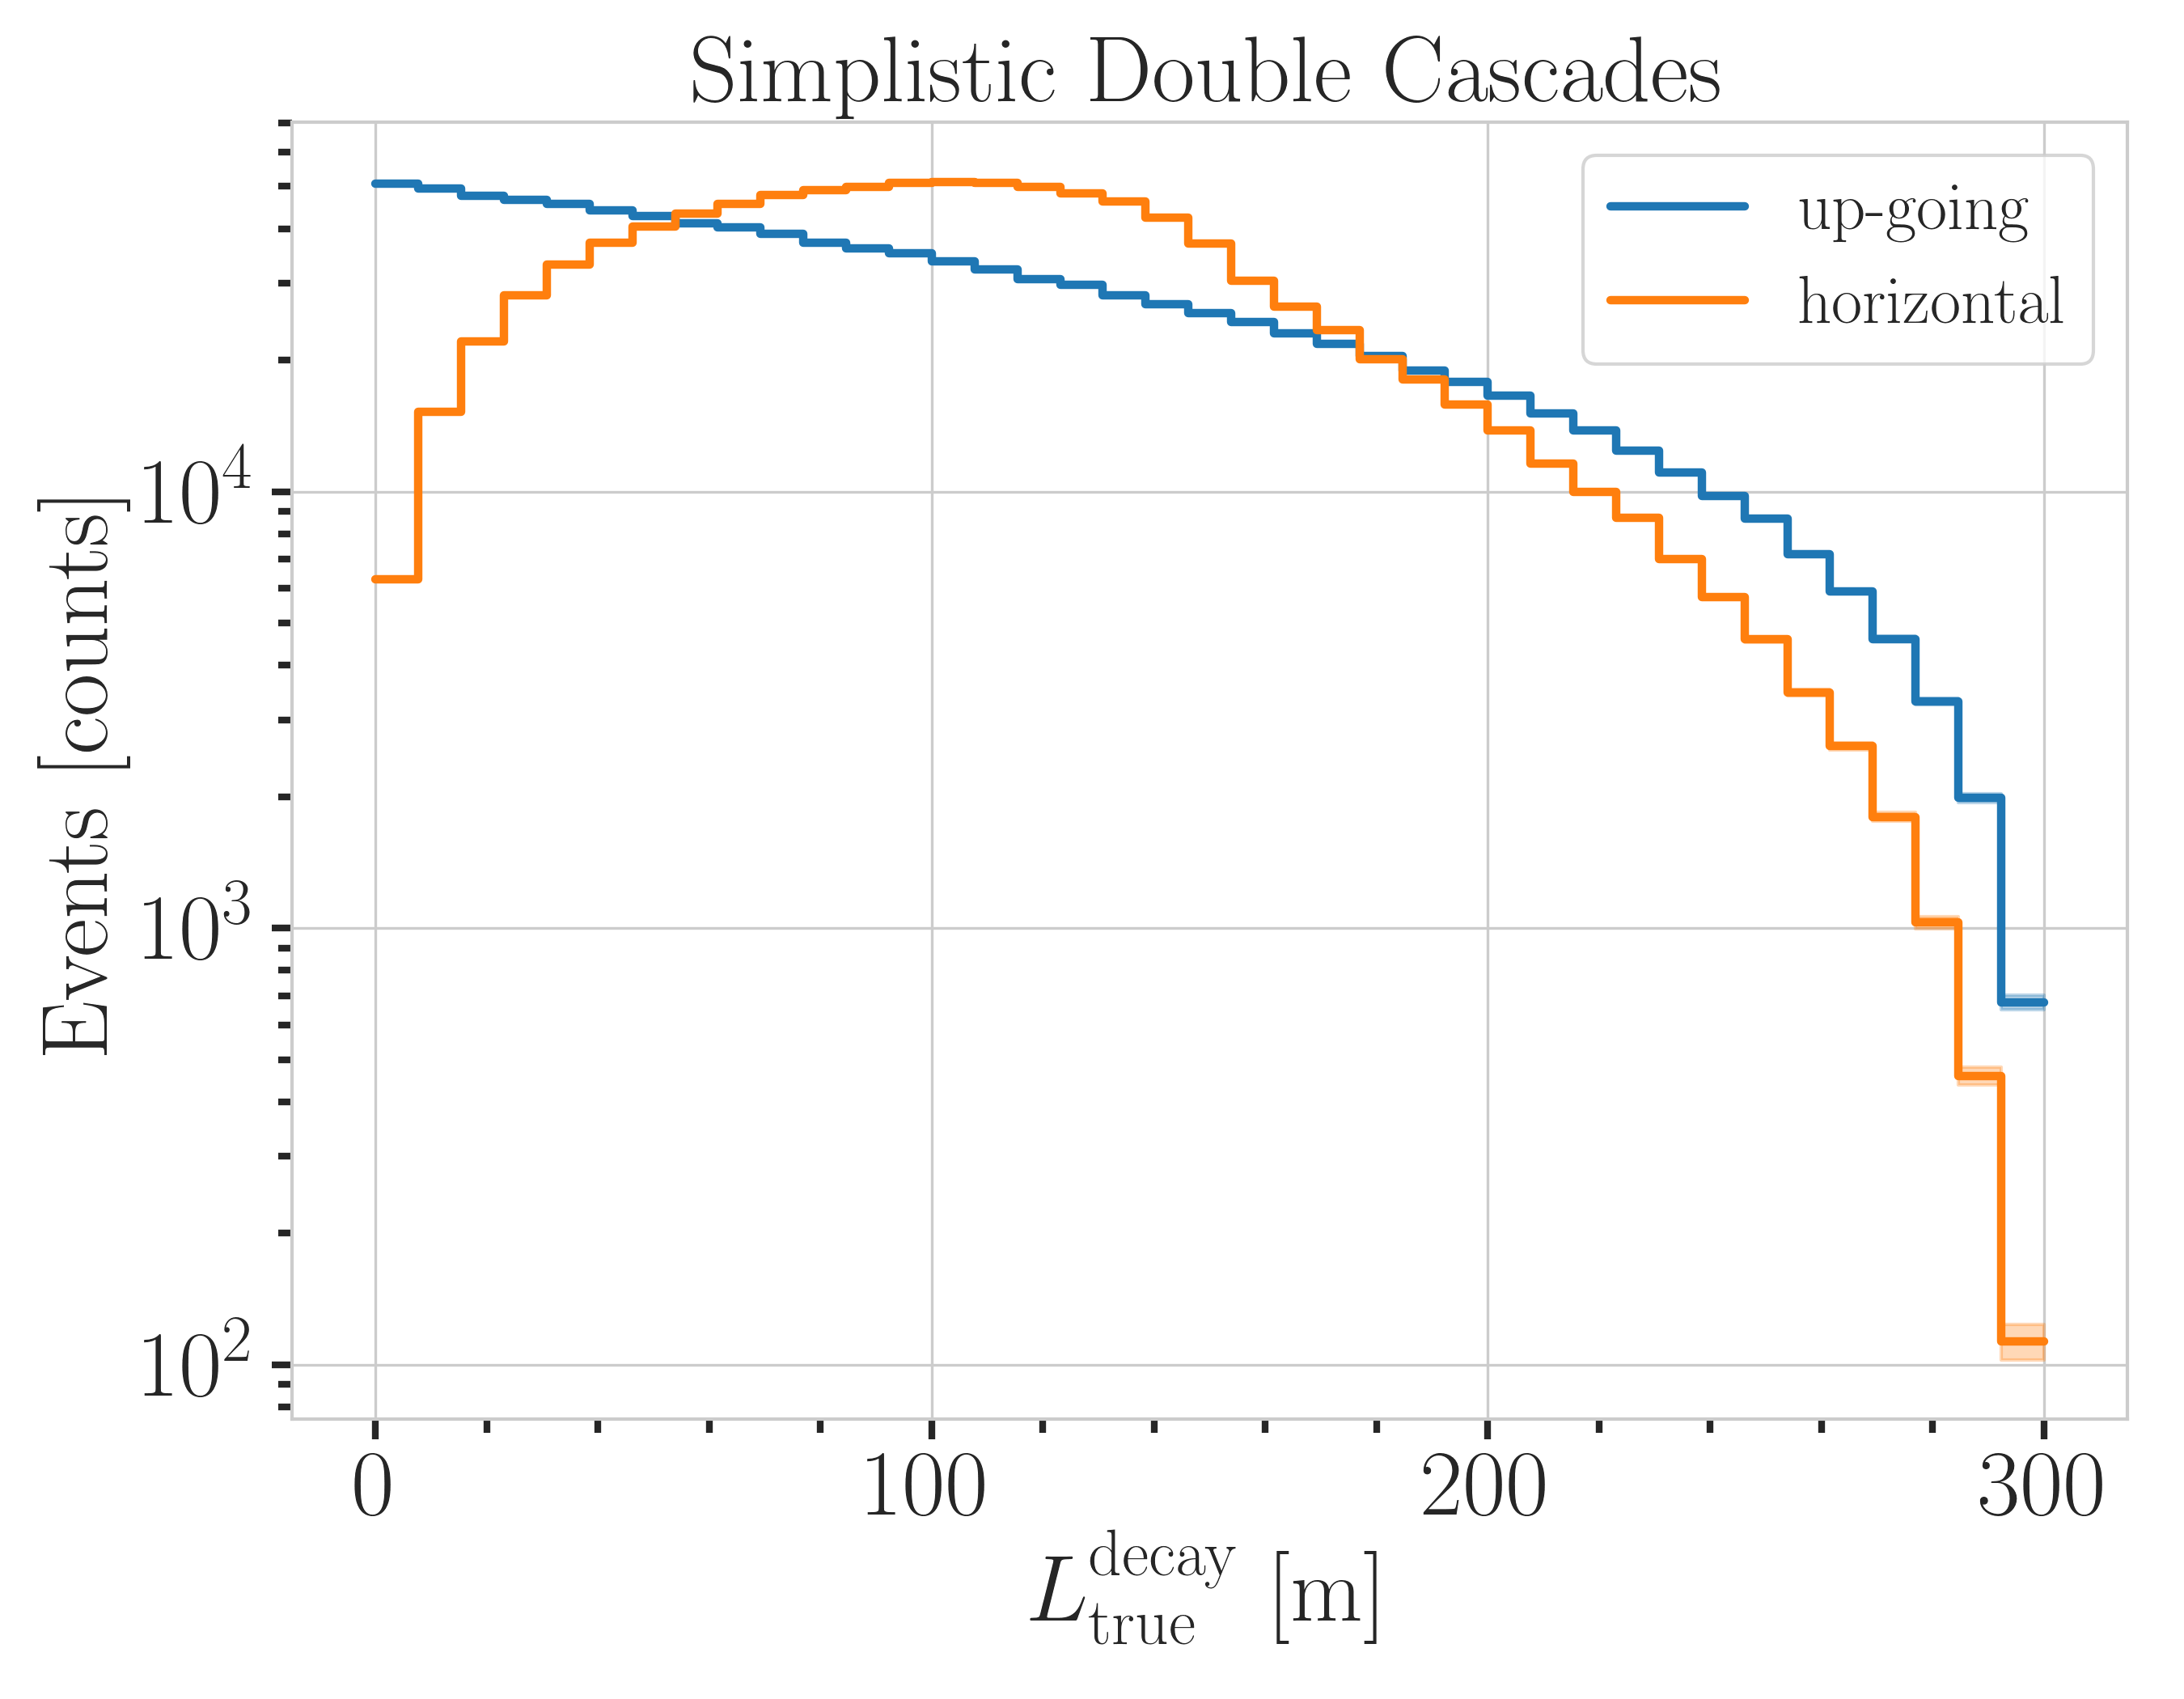
\includegraphics[width=.49\linewidth]{figures/model_independent_simulation/gen_level/simplistic_1_d_distr_true_decay_length.png}
    \caption[Simplified model-independent simulation generation level distributions]{Generation level distributions of the simplistic simulation samples. Cascade and total energies (left) and decay lengths (right) of both samples are shown.}
    \labfig{simplified_gen_distris}
\end{figure*}

The second sample is used to investigate the reconstruction performance for horizontal events, where the spacing between DOMs is much larger. The cascades are placed uniformly on a circle with radius of $r=\SI{150}{\meter}$ centered in DeepCore at the depth of $z=\SI{-330}{\meter}$. The direction is always horizontal and azimuth is defined by the connecting vector of both cascade positions. The energies are again sampled uniformly between \SIrange[range-phrase={~and~}]{0.0}{60.0}{\gev}. The specific sampling distributions/values for the cascades are listed in \reftab{hnl_simplified_sampling_distributions}, for both samples and for completeness, all distributions are shown in \reffig{realistic_gen_distris_appendix}.

\begin{table}[h]
    \small
        \begin{tabular}{ llll }
        \hline\hline
        \textbf{Sample} & \textbf{Variable} & \textbf{Distribution} & \textbf{Range/Value} \\
        \hline\hline
        \multicolumn{2}{l}{Up-going} && \\
        \hline
        & energy & uniform & \SIrange{0.0}{60.0}{\gev} \\
        & zenith & fixed & \SI{180.0}{\degree} \\
        & azimuth & fixed & \SI{0.0}{\degree} \\
        & $x,y$ position & fixed & (41.6, 35.49)\,\si{\metre} \\
        & $z$ position & uniform & \SIrange{-480.0}{-180.0}{\metre} \\
        \hline
        \multicolumn{2}{l}{Horizontal} && \\ 
        \hline
        & energy & uniform & \SIrange{0.0}{60.0}{\gev} \\
        & zenith & fixed & \SI{90.0}{\degree} \\
        & azimuth & uniform & \SIrange{0.0}{360.0}{\degree} \\
        & $x,y$ position & uniform (circle) & $c$=(46.29, -34.88)\,\si{\metre}, $r$=\SI{150.0}{\metre} \\
        & $z$ position & fixed & \SI{-330.0}{\metre} \\
        \hline
        \end{tabular}
    \caption[Simplified model-independent simulation sampling distributions]{Generation level sampling distributions and ranges/values of up-going and horizontal model-independent simulation.}
    \labtab{hnl_simplified_sampling_distributions}
\end{table}



\subsection{Realistic Sample} \labsec{realistic_sample}

To thoroughly investigate the potential of IceCube DeepCore to detect double cascade events, a more realistic simulation sample is produced that aims to be as close as possible to the expected signal simulation explained in \refsec{model_specific_simulation}, while still allowing additional freedom to control the double cascade kinematics. This sample is particularly useful for validating the model-dependent HNL simulation described in \refsec{model_specific_simulation}.

For this purpose the total energy is sampled from an $E^{-2}$ power law, mimicking the energy spectrum of the primary neutrinos as stated in \refsec{neutrino_generation}. The total energy is divided into two parts, by assigning a fraction between \SIrange[range-phrase={~and~}]{0}{100}{\percent} to one cascade and the remaining part to the other cascade. This is a generic approximation of the realistic process described in \refsec{model_specific_simulation}, and chosen such that the whole sample covers various cases of energy distributions between the two cascades. The decay length is sampled from an exponential distribution, as expected for a decaying heavy mass state. The resulting energy distributions and the decay length distribution are shown in \reffig{realistic_gen_distris}, where it can be seen that the individual cascade energies can be very small, due to splitting the total energy, and the decay lengths spans across several orders of magnitude.

\begin{figure*}[h]
    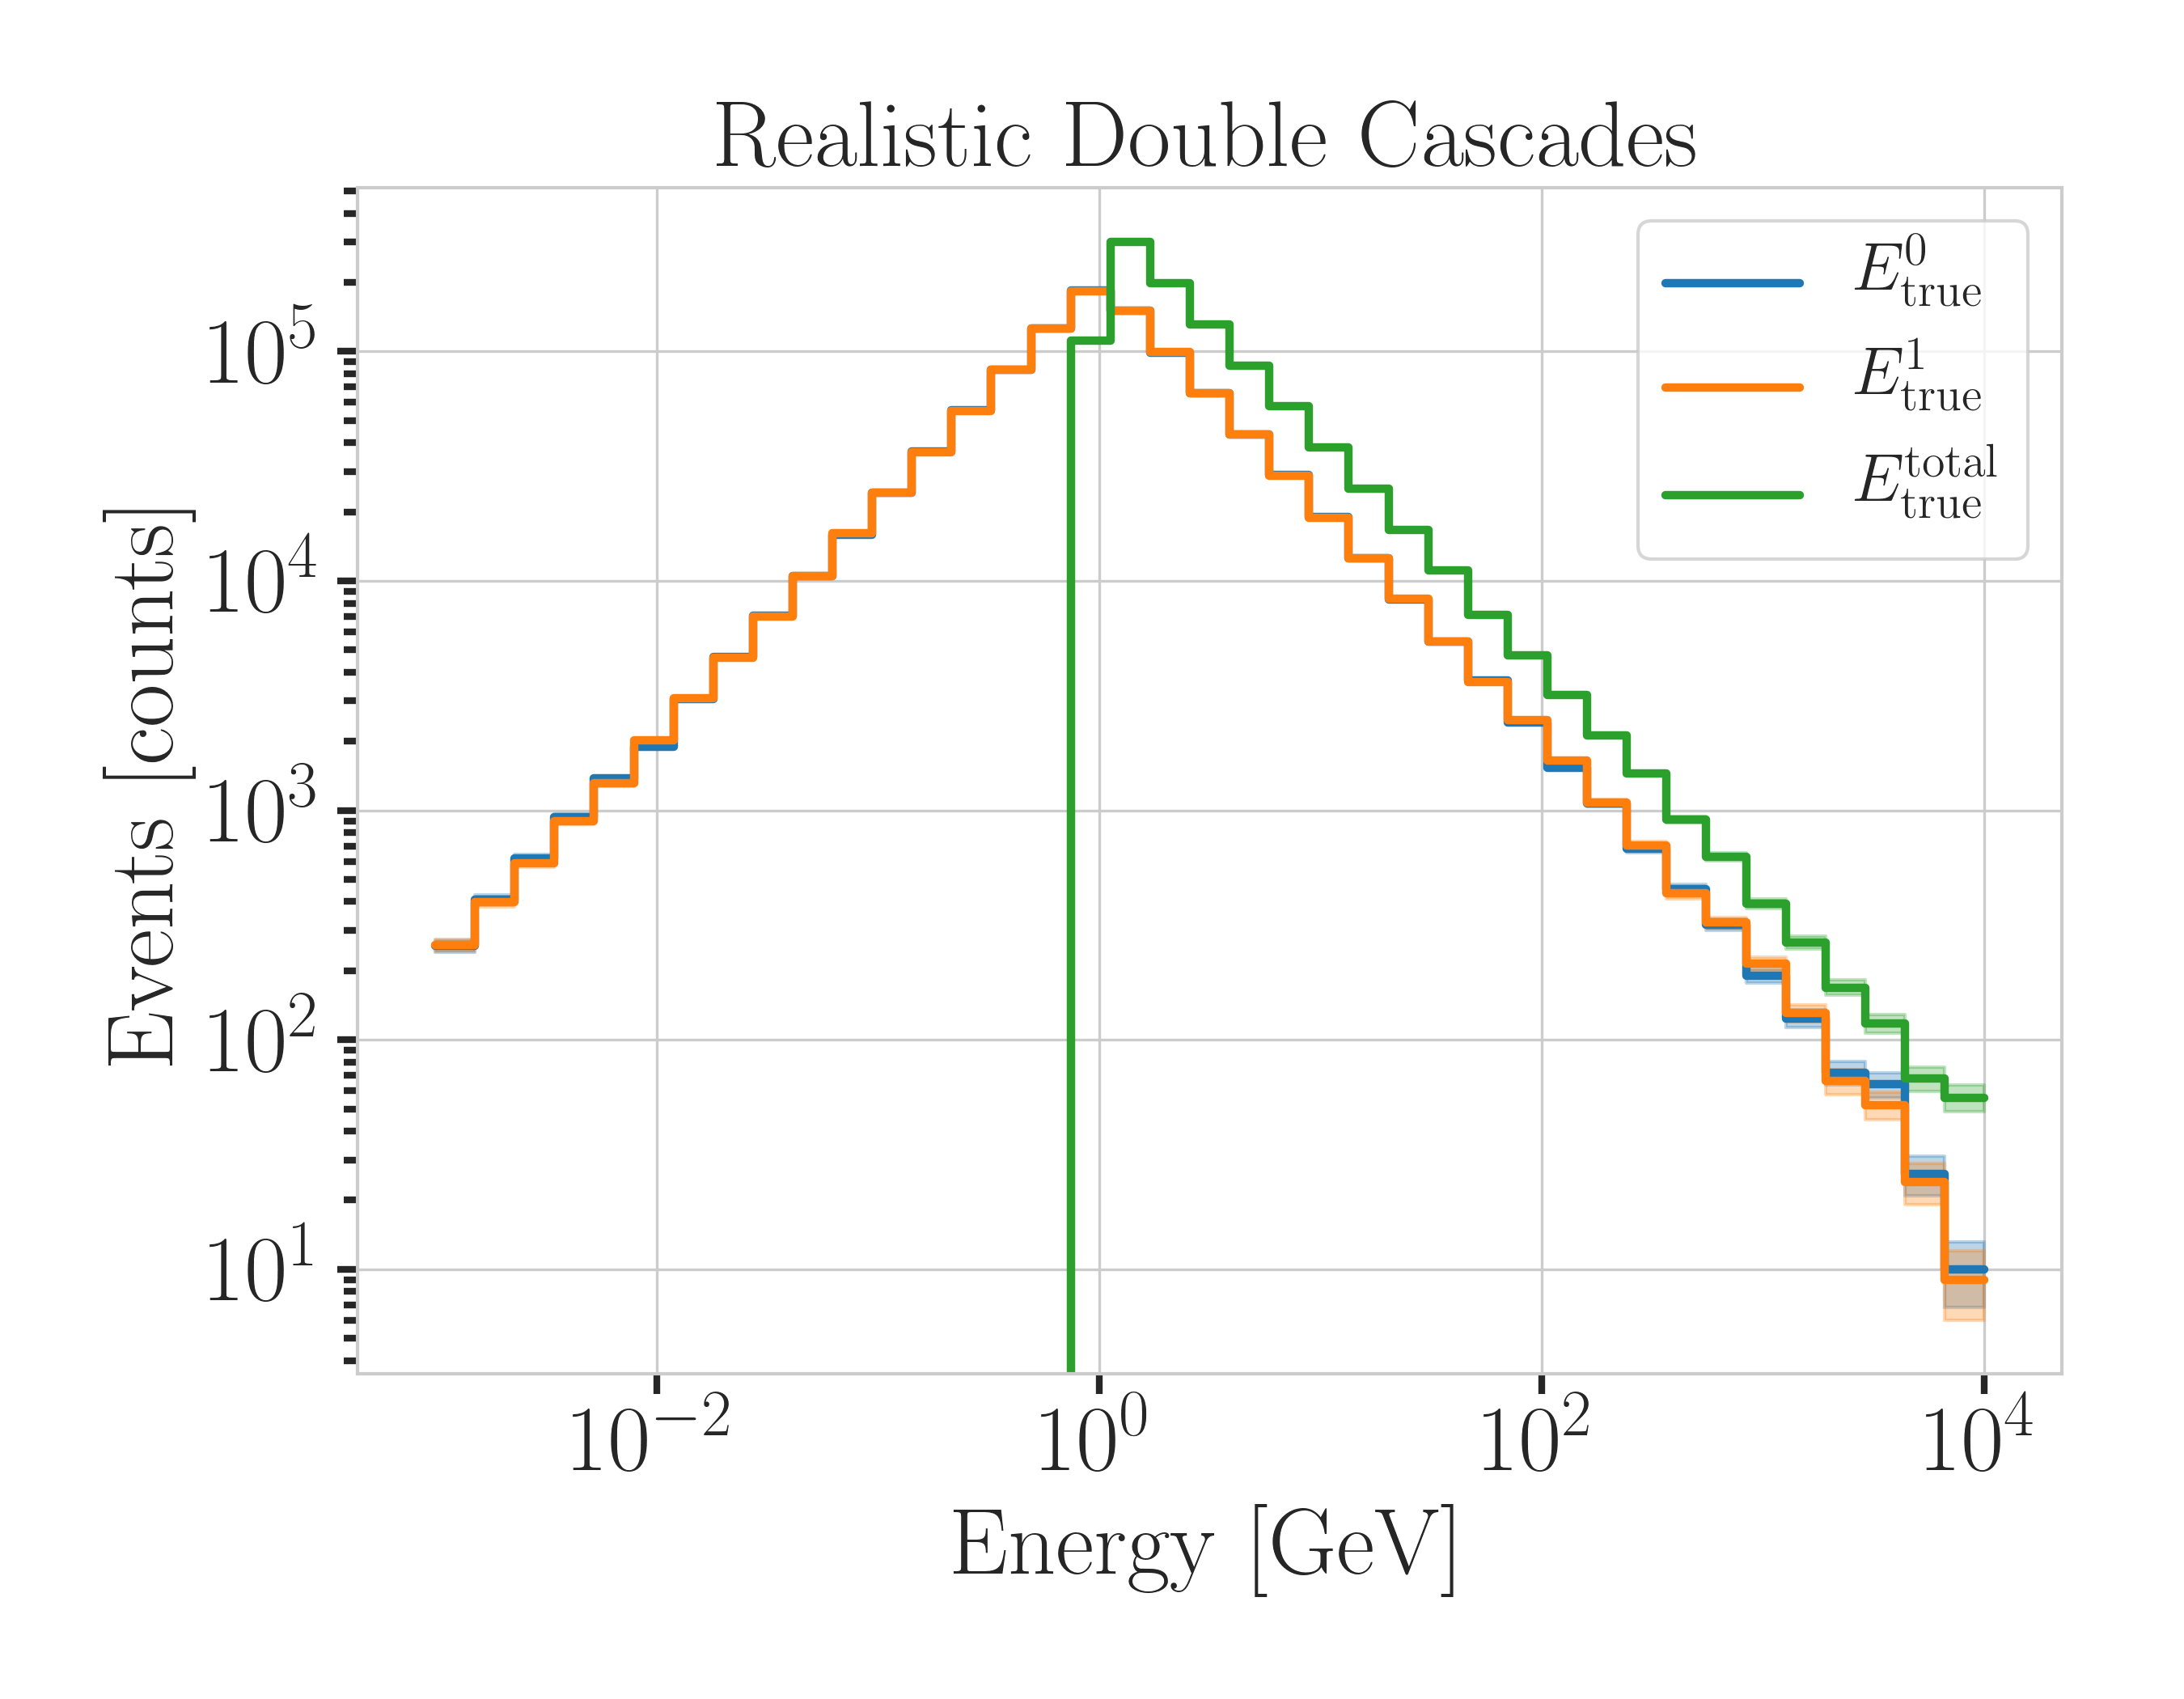
\includegraphics[width=.49\linewidth]{figures/model_independent_simulation/gen_level/194603_gen_level_1_d_distr_all_energies.png}
    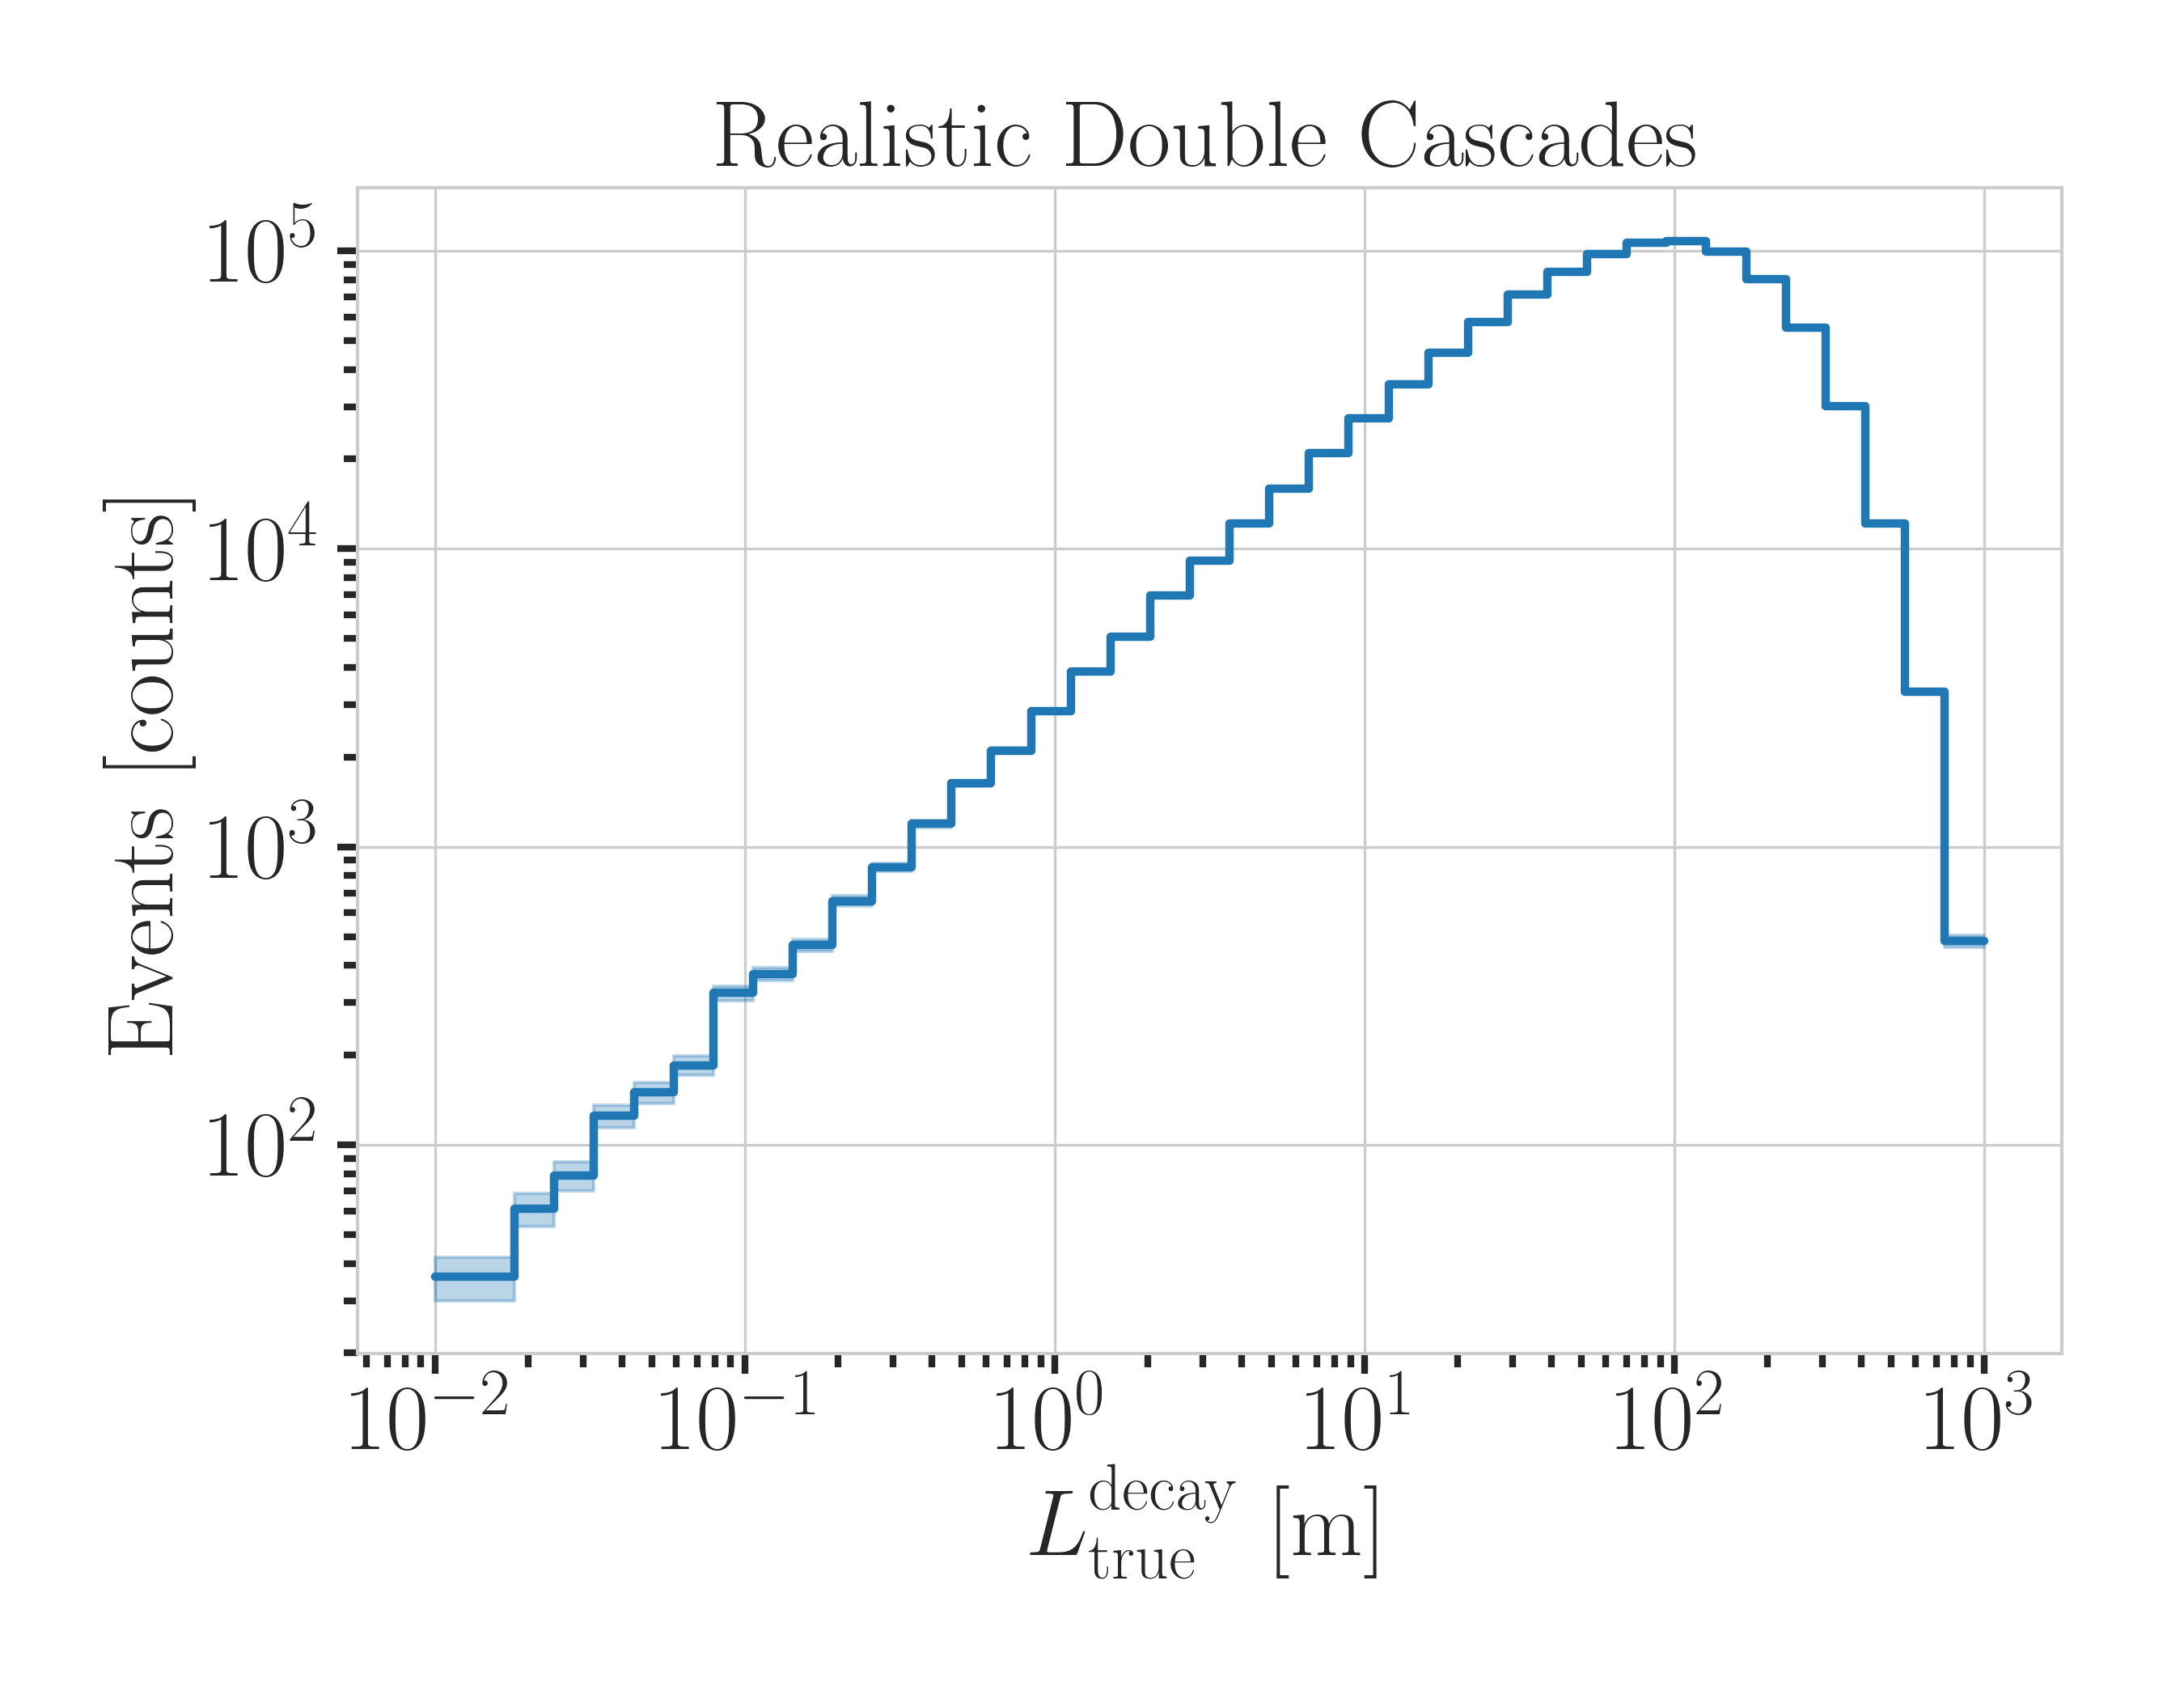
\includegraphics[width=.49\linewidth]{figures/model_independent_simulation/gen_level/194603_gen_level_1_d_distr_true_decay_length.png}
    \caption[Realistic model-independent simulation generation level distributions]{Generation level distributions of the realistic sample. Shown are the individual cascade energies and total energy (left) and decay lengths (right). It can be seen how the cascade energies can get very small, and the decay length follows a more realistic distribution spanning across several orders of magnitude.}
    \labfig{realistic_gen_distris}
\end{figure*}

To efficiently generate events in a way that produces distributions similar to what would be observed with DeepCore, one of the cascade positions is sampled inside the DeepCore volume by choosing its coordinates uniformly on a cylinder that is centered in DeepCore. This is similar to a trigger condition of one cascade always being inside the DeepCore fiducial volume. Choosing the direction of the event by sampling zenith and azimuth uniformly between \SIrange[range-phrase={~and~}]{70}{180}{\degree} and \SIrange[range-phrase={~and~}]{0}{360}{\degree}, respectively, the position of the other cascade can be inferred for a given decay length, assuming a travel speed of $c$, and choosing whether the cascade position that was sampled is the first cascade or the second with a \SI{50}{\percent} chance. The zenith angle is chosen between straight up-going (zenith of \SI{180}{\degree}) and slightly down-going from above the horizon (\SI{70}{\degree}) to mimic an event selection that reduces atmospheric muons by rejecting events coming from above the horizon, but still incorporates some down-going events. All distributions are shown in \reffig{realistic_gen_distris_appendix}, and the sampling distributions/values are listed in \reftab{hnl_realistic_sample_sampling_distributions}.

\begin{table}[h]
    \small
        \begin{tabular}{ llll }
        \hline\hline
        \textbf{Variable} & \textbf{Distribution} & \textbf{Range/Value} \\
        \hline\hline
        energy (total) & power law $E^{-2}$ & \SIrange{1}{1000}{\gev} \\
        decay length & exponential e$^{-0.01L}$ & \SIrange{0}{1000}{\metre} \\
        zenith & uniform & \SIrange{70}{180}{\degree} \\
        azimuth & uniform & \SIrange{0}{360}{\degree} \\
        $x,y$ (one cascade) & uniform (circle) & $c$=(46.29, -34.88)\,\si{\metre}, $r$=\SI{150}{\metre} \\
        $z$ (one cascade) & uniform & \SIrange{-480.0}{-180.0}{\metre}\\
        \hline
        \end{tabular}
        \caption[Realistic model-independent simulation sampling distributions]{Generation level sampling distributions and ranges/values of the realistic model-independent simulation.}
    \labtab{hnl_realistic_sample_sampling_distributions}
\end{table}


\section{Model-Dependent Heavy Neutral Lepton Event Generation} \labsec{model_specific_simulation}

To estimate the HNL event expectation in IceCube DeepCore, depending on the specific model parameters, a generator was developed that is based on the HNL theory introduced in \refsec{hnl_theory}. For this work, only the interaction with the $\tau$-sector was taken into account ($|U_{\alpha4}^2|=0$, $\alpha=e,\mu$), which reduces the physics parameters of interest and relevant for the generation to the fourth heavy lepton mass, $m_4$, and the mixing, $|U_{\tau4}^2|$.

Due to the very low interaction rate of neutrinos, which are the source of HNL production, the event generation is performed in a way that forces every event to interact in a chosen sampling volume. The weight of each event is then calculated as the inverse of the simulated neutrino fluence
\begin{equation}
    w_\rm{gen} = \frac{1}{F_{\mathrm{sim}}} \frac{1}{N_{\mathrm{sim}}}
    \;,
    \labeq{neutrino_generation_weight}
\end{equation}
where $F_{\rm{sim}}$ is the number of neutrino events per energy, time, area, and solid angle, and $N_{\rm{sim}}$ is the number of simulated events. If this weight is multiplied by the livetime and the theoretically expected neutrino flux for a given physical model, it results in the number of expected events in the detector for this particular MC event.

The generator uses a customized \textit{\textsc{LeptonInjector} (LI)} version to create the events and \textit{\textsc{LeptonWeighter} (LW)} to weight them \sidecite{IceCube:2020tcq}. The modified LI and the essential components needed for the HNL simulation are described in the next sections, followed by the description of the weighting scheme and the sampling distributions chosen for the generation.


\subsection{Custom LeptonInjector} \labsec{custom_leptoninjector}

In its standard version, the LI generator produces neutrino interactions by injecting a lepton and a hadronic cascade at the interaction vertex of the neutrino, where the lepton is the charged (neutral) particle produced in a CC (NC) interaction and the cascade is the hadronic cascade from the nucleus that is breaking apart. The hadronic cascade is stored as a specific object of type \textit{Hadrons}, which triggers the correct simulation of the shower development in the following simulation steps. Below \SI{30}{\gev} the individual hadrons are simulated using \textsc{Geant4} \sidecite{geant4} while for higher energies an analytical approximation from \sidecite{raedel_wiebusch_cherenkov_yield} is used. The main differences to an EM cascade is that part of the energy will not be observed, because it goes into neutral particles, and that the spatial development of the shower is different as discussed in \refsec{hadronic_showers}. Both objects are injected with the same $(x,y,z,t)$ coordinates and the kinematics are sampled from the differential and total cross-sections that are one of the inputs to LI.

\begin{figure}[h]
    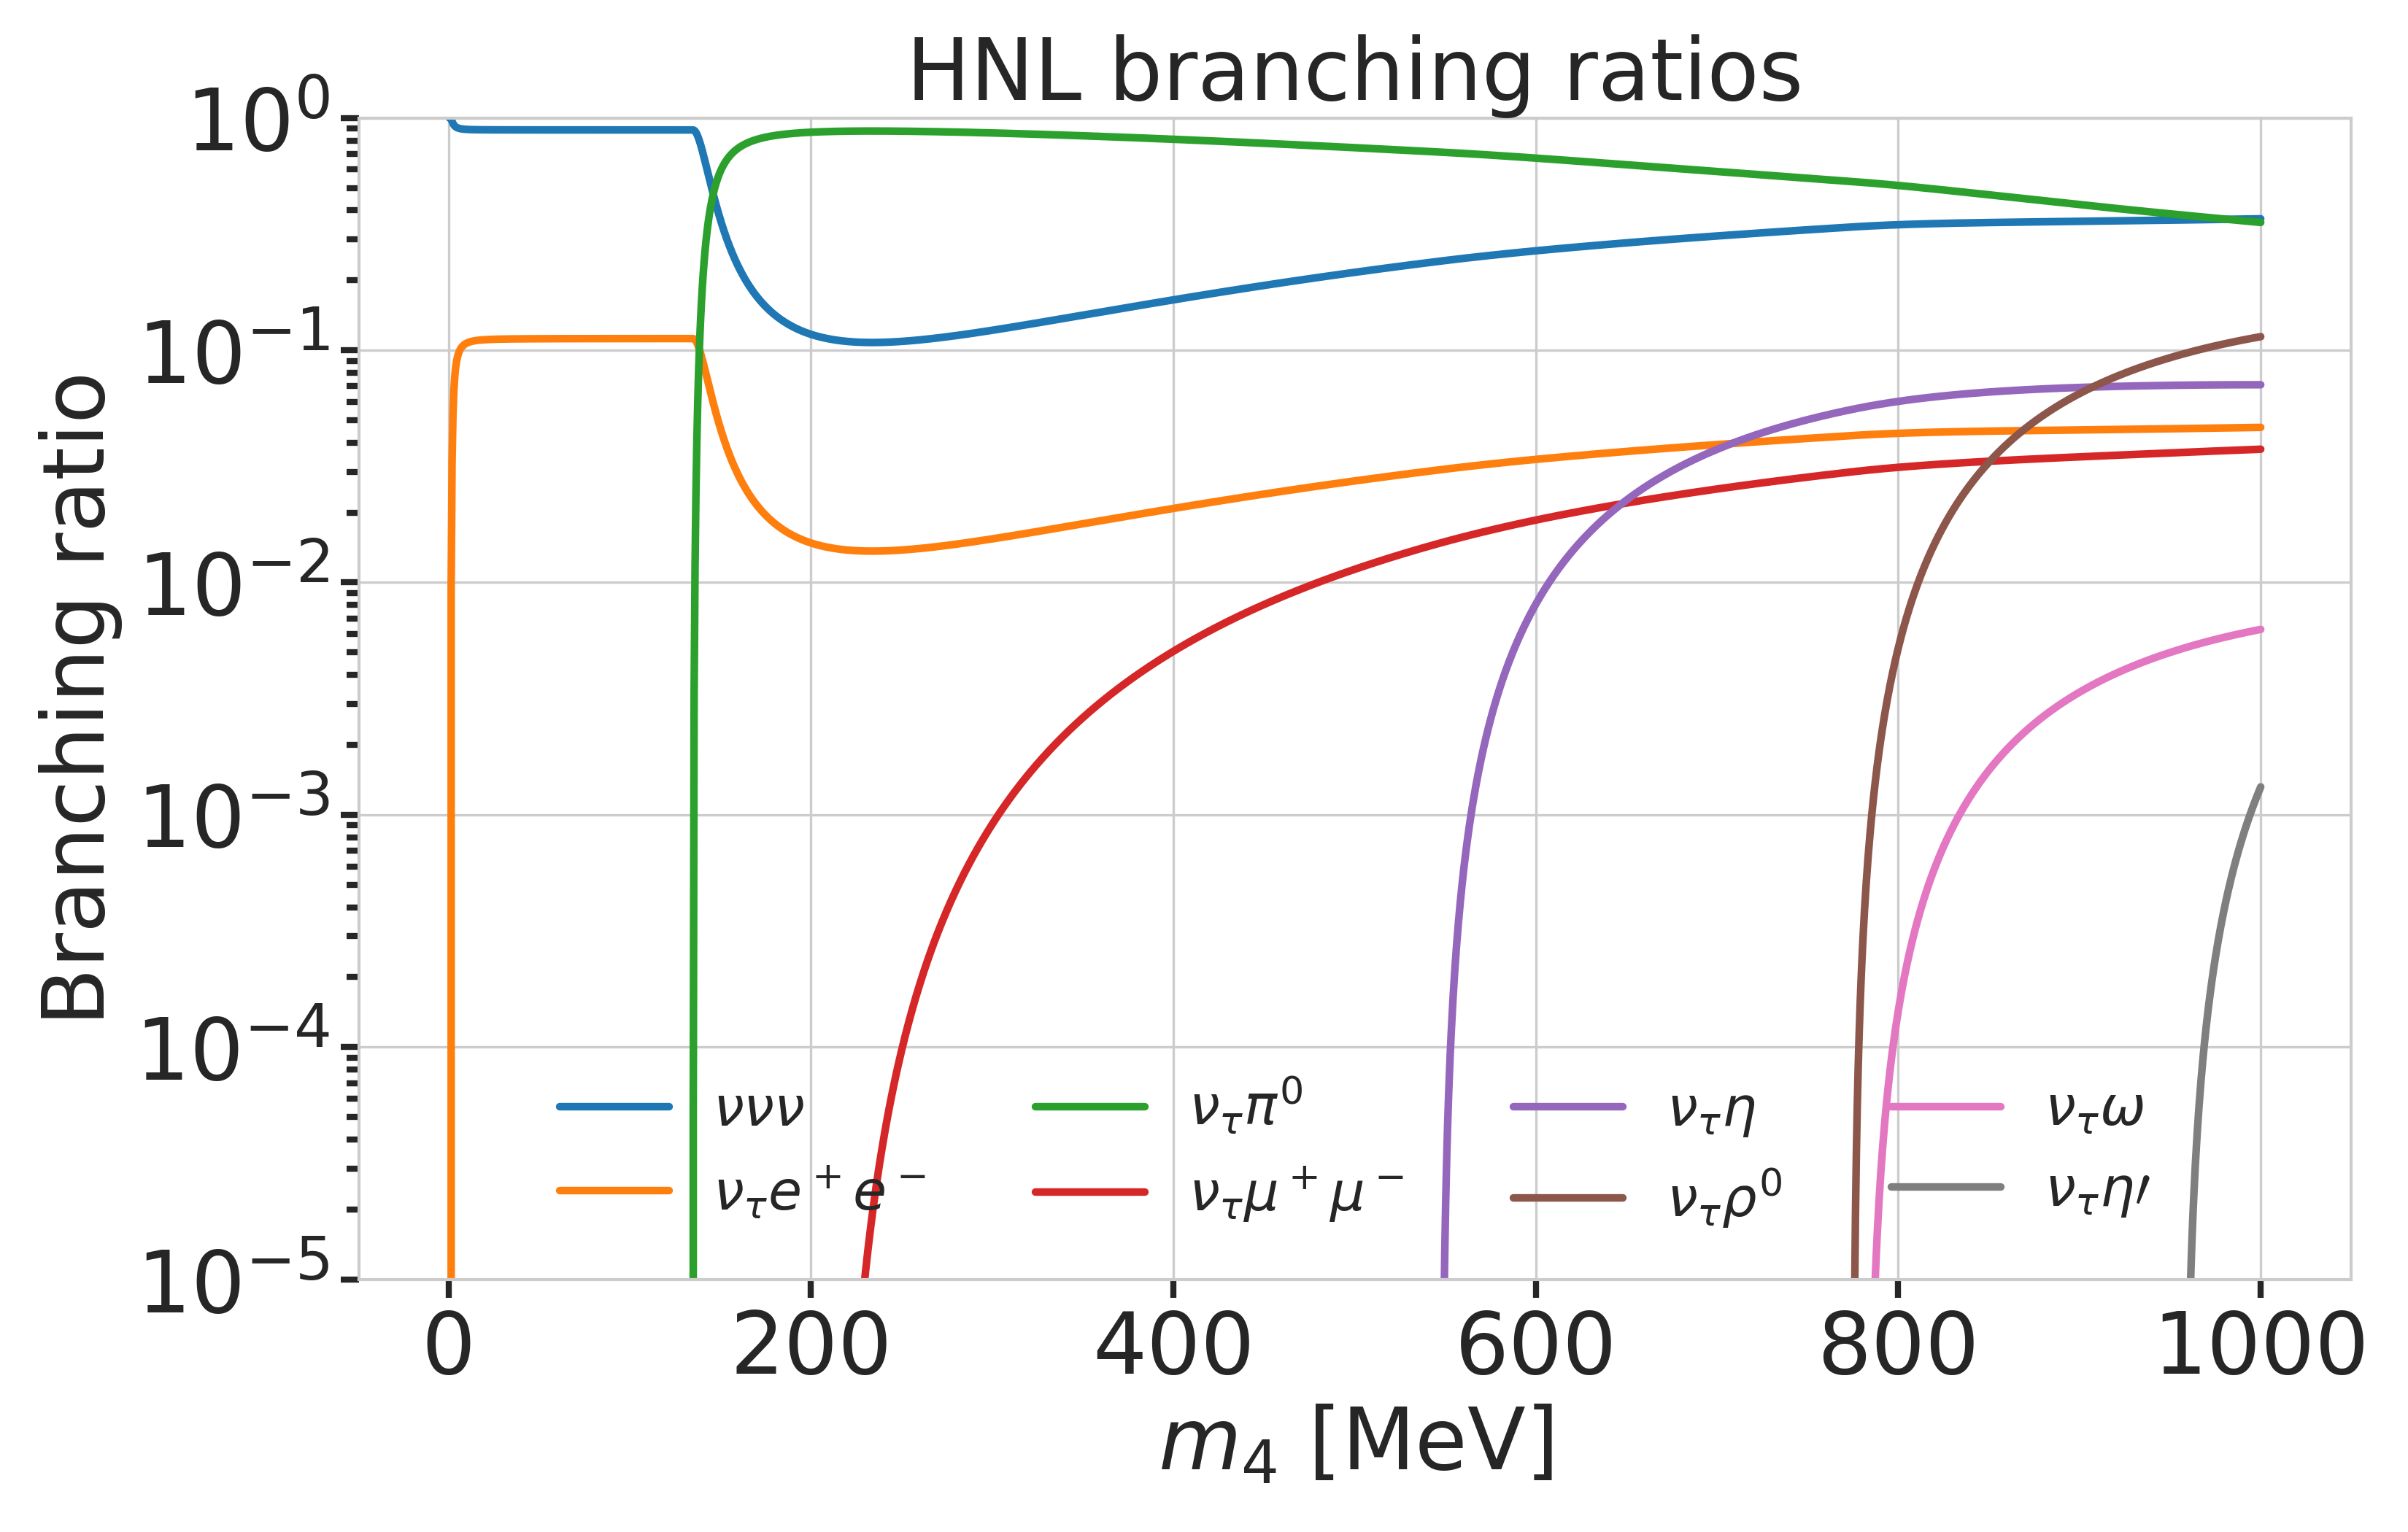
\includegraphics{hnl_simulation/decay_theory/branching_ratios_linear_up_to_1.0_GeV.png}
    \caption[HNL branching ratios]{Branching ratios of the HNL within the mass range considered in this work, only considering $|U_{\tau4}^2| \neq 0$, calculated based on the results from \cite{Coloma:2020lgy}.}
    \labfig{hnl_branching_ratios}
\end{figure}

In the modified version, the SM lepton at the interaction vertex is replaced by the new HNL particle, where the interaction cross-sections are replaced by custom, mass dependent HNL cross-sections. The HNL is forced to decay after a chosen distance\sidenote{The explicit sampling distributions and ranges can be found in \refsec{hnl_sampling_distributions}.} to produce secondary SM particles, where the decay mode is chosen with a probability given by the mass dependent branching ratios from the kinematically accessible decay modes shown in \reffig{hnl_branching_ratios}. The cross-section and decay width calculations were implemented for this purpose and will be explained in more detail in the following. Another addition to LI is that the decay products of the HNL are also stored. These HNL daughter particles form the second cascade, not as a single hadronic cascade object, but as the explicit particles forming the shower. They are injected with the correctly displaced position and delayed time from the interaction vertex, given the HNL decay length. The kinematics of the two-body decays are computed analytically, while the 3-body decay kinematics are calculated with \textsc{MadGraph} \sidecite{madgraph}, which will also be explained further below. Independent of the number of particles in the final state of the HNL decay, the kinematics are calculated/simulated at rest and then boosted along the HNL momentum.

Muons produced in those decays are propagated using \textsc{Proposal} \sidecite{proposal}, also simulating their Cherenkov light output. The shower development of gamma rays, electrons, and positrons below \SI{100}{\mega\electronvolt} is also simulated using Geant4 and for higher energies the analytical approximation is used again \cite{raedel_wiebusch_cherenkov_yield}.

The injection is done using the LI \textit{volume mode}, for the uniform injection of the primary particle on a cylindrical volume, adding \SI{50}{\percent} of the events with $\nu_\tau$ and the other half with $\bar{\nu}_\tau$ as primary particle types. The generator takes the custom double-differential/total cross-section splines described below and the parameters defining the sampling distributions as inputs.


\subsubsection{Cross-Sections}

The cross-sections are calculated using the \textsc{NuXSSplMkr} \cite{xsecmaker} software, which is a tool to calculate neutrino cross-sections from \textit{parton distribution functions (PDFs)} and then fit to an N-dimensional tensor-product B-spline surface \sidecite{photospline} to produce the splines that can be read and used with LI/LW. The tool was modified to produce the custom HNL cross-sections, where the main modification to calculate the cross-sections for the $\nu_\tau$-NC interaction into the new heavy mass state, is the addition of a kinematic condition to ensure that there is sufficient energy to produce the heavy mass state. It is the same condition fulfilled for the CC case, where the outgoing charged lepton mass is non-zero. Following \sidecite{Levy:2004rk} (equation 7), the condition
\begin{equation}
    (1 + x \delta_N) h^2 - (x + \delta_{4}) h + x \delta_{4} \leq 0
    \;
    \labeq{hnl_kinematic_condition}
\end{equation}
is implemented for the NC case in the NuXSSplMkr code. Here
\begin{align}
    \delta_{4} ={}& \frac{m_4^2}{s-M^2}
    \;, \\
    \delta_{N} ={}& \frac{M^2}{s-M^2}
    \;, \rm{and} \\
    h \overset{\textit{def}}{=}& xy + \delta_{4}
    \;,
    \labeq{hnl_kinematic_condition_variables}
\end{align}
with $x$ and $y$ being the Bjorken variables, $m_4$ and $M$ the mass of the heavy state and the target nucleon, respectively, and $s$ the center of mass energy squared. The custom version was made part of the open source NuXSSplMkr software and can thus be found in \cite{xsecmaker}. The result of this kinematic condition is that events cannot be produced for energy, $x$, $y$ combinations that do not have sufficient energy to produce the outgoing, massive lepton. This results in a reduction of the cross-section towards lower energies, which scales with the assumed mass of the HNL. This effect can be seen in \reffig{custom_hnl_cross_sections}.

\begin{figure*}[h]
    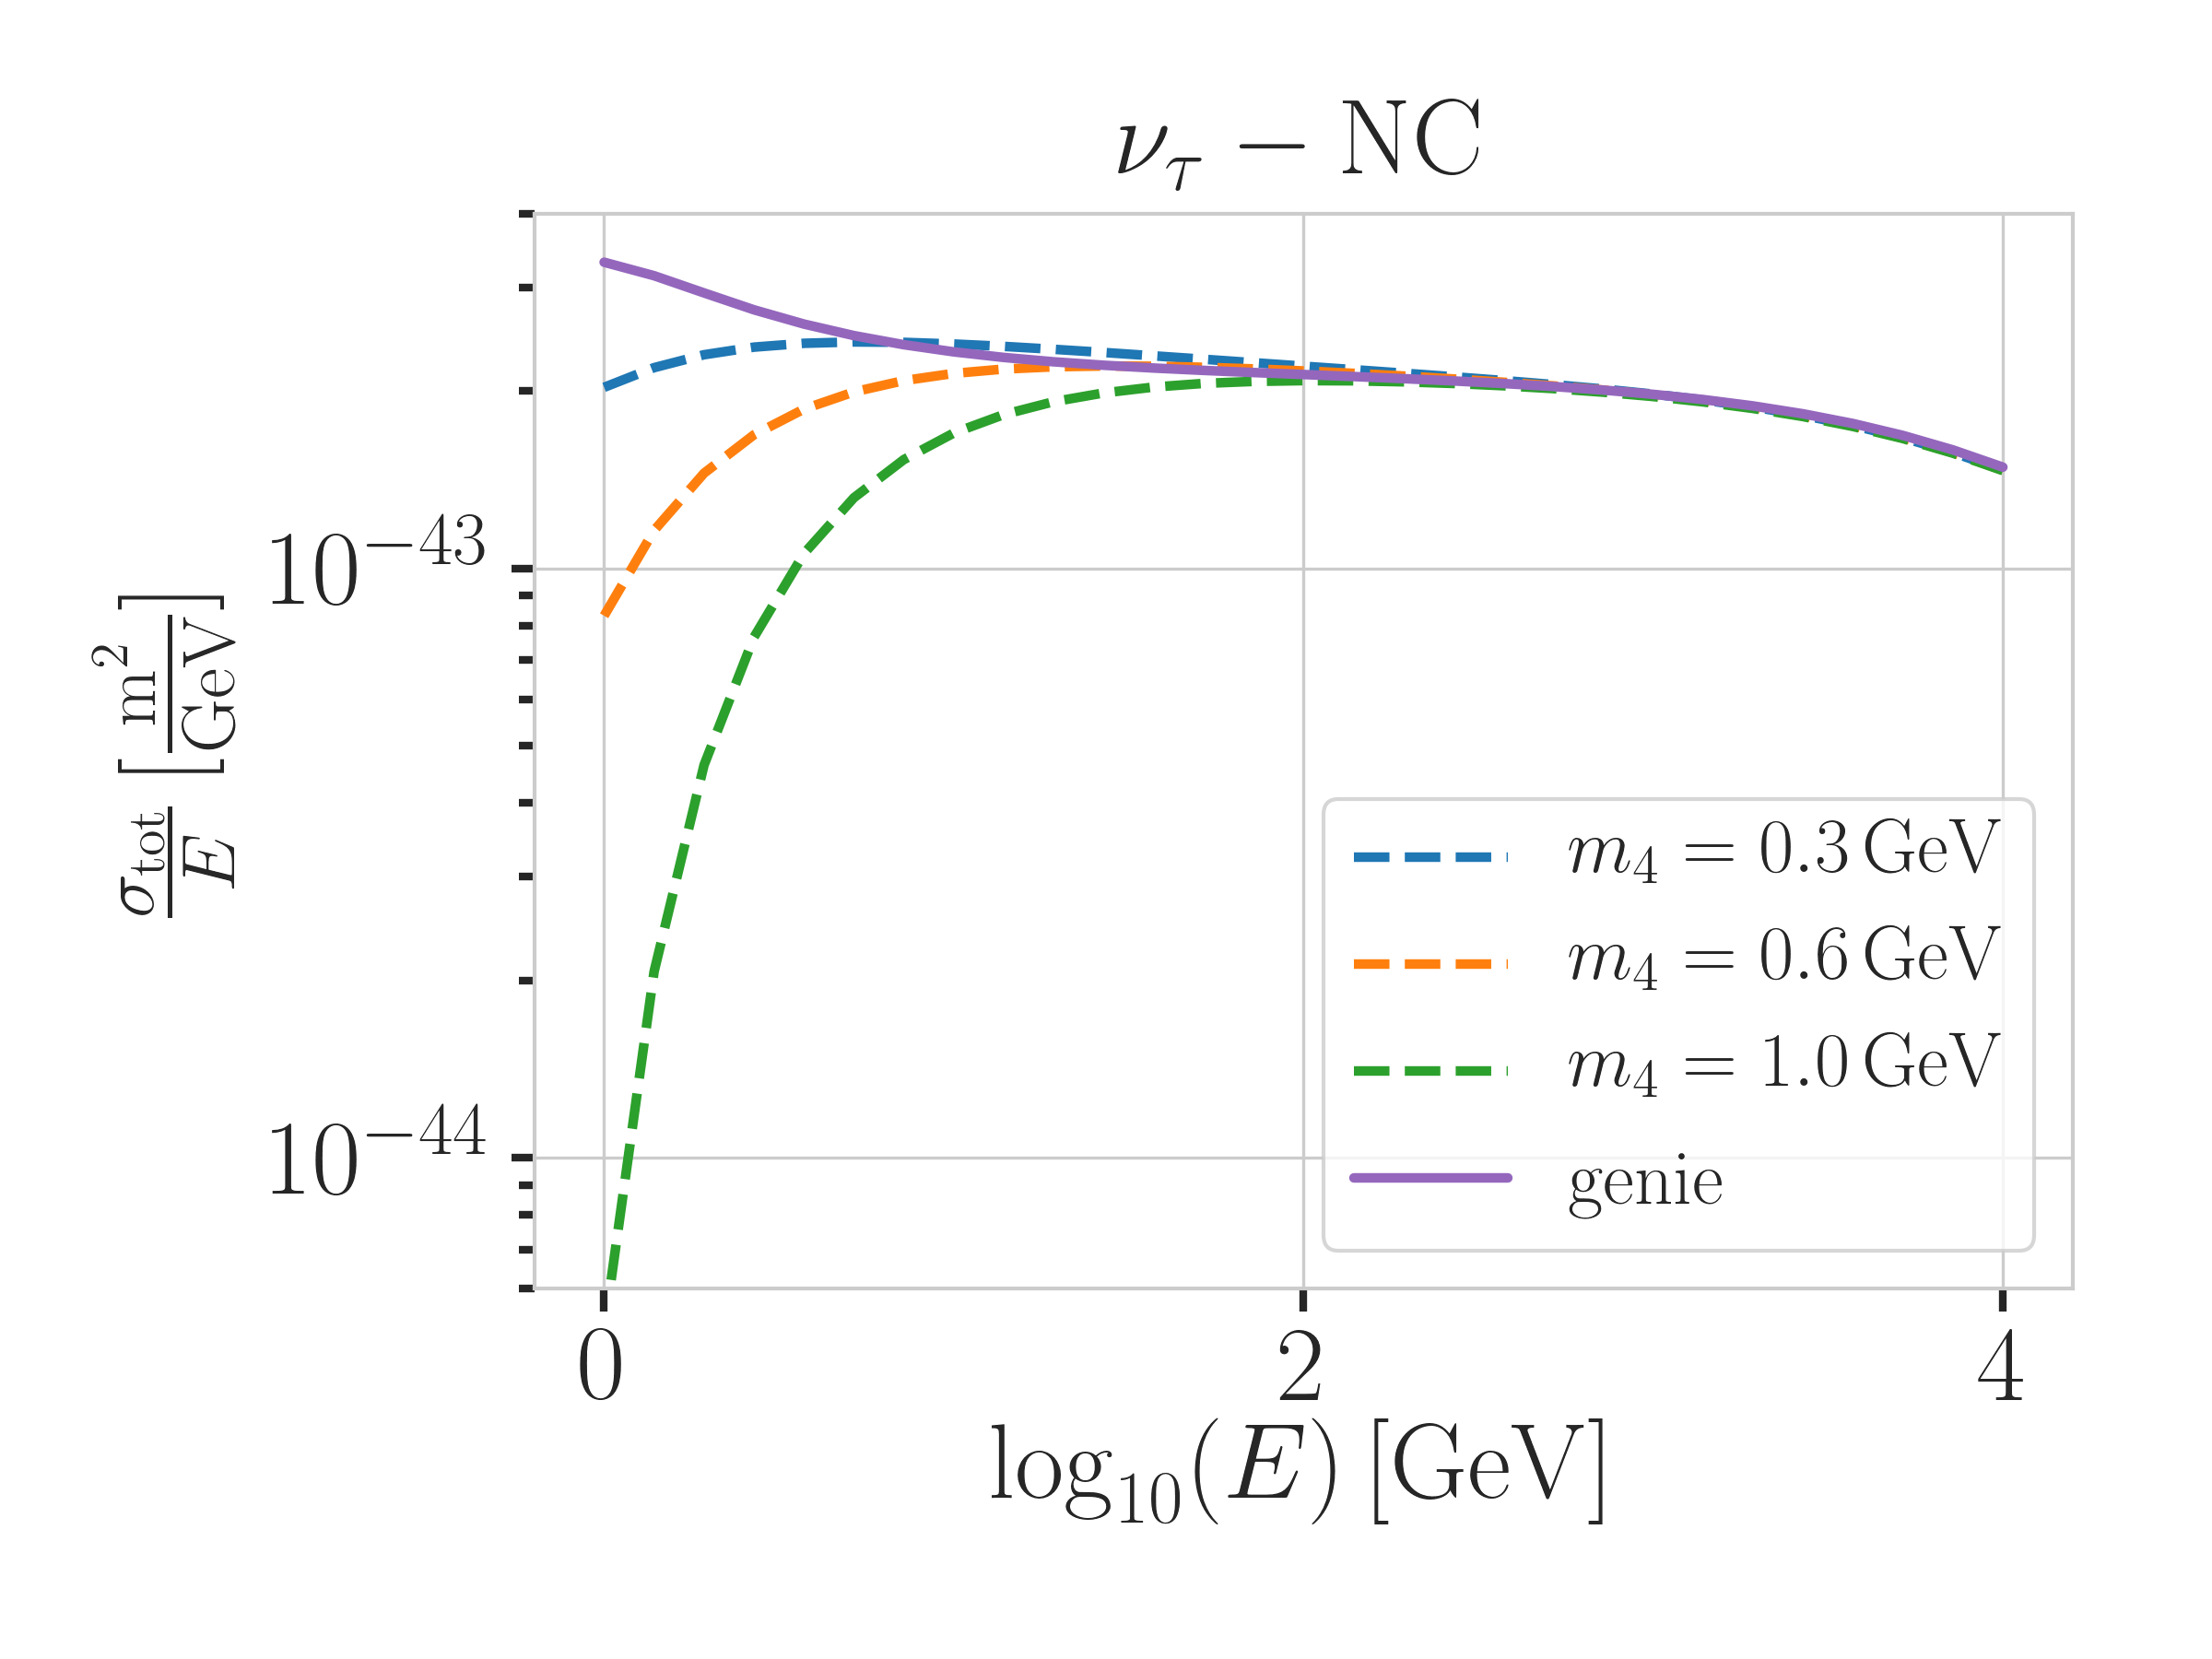
\includegraphics[width=.49\linewidth]{figures/hnl_simulation/cross_sections/custom_HNL_thesis_sigma-nutau-N-nc.png}
    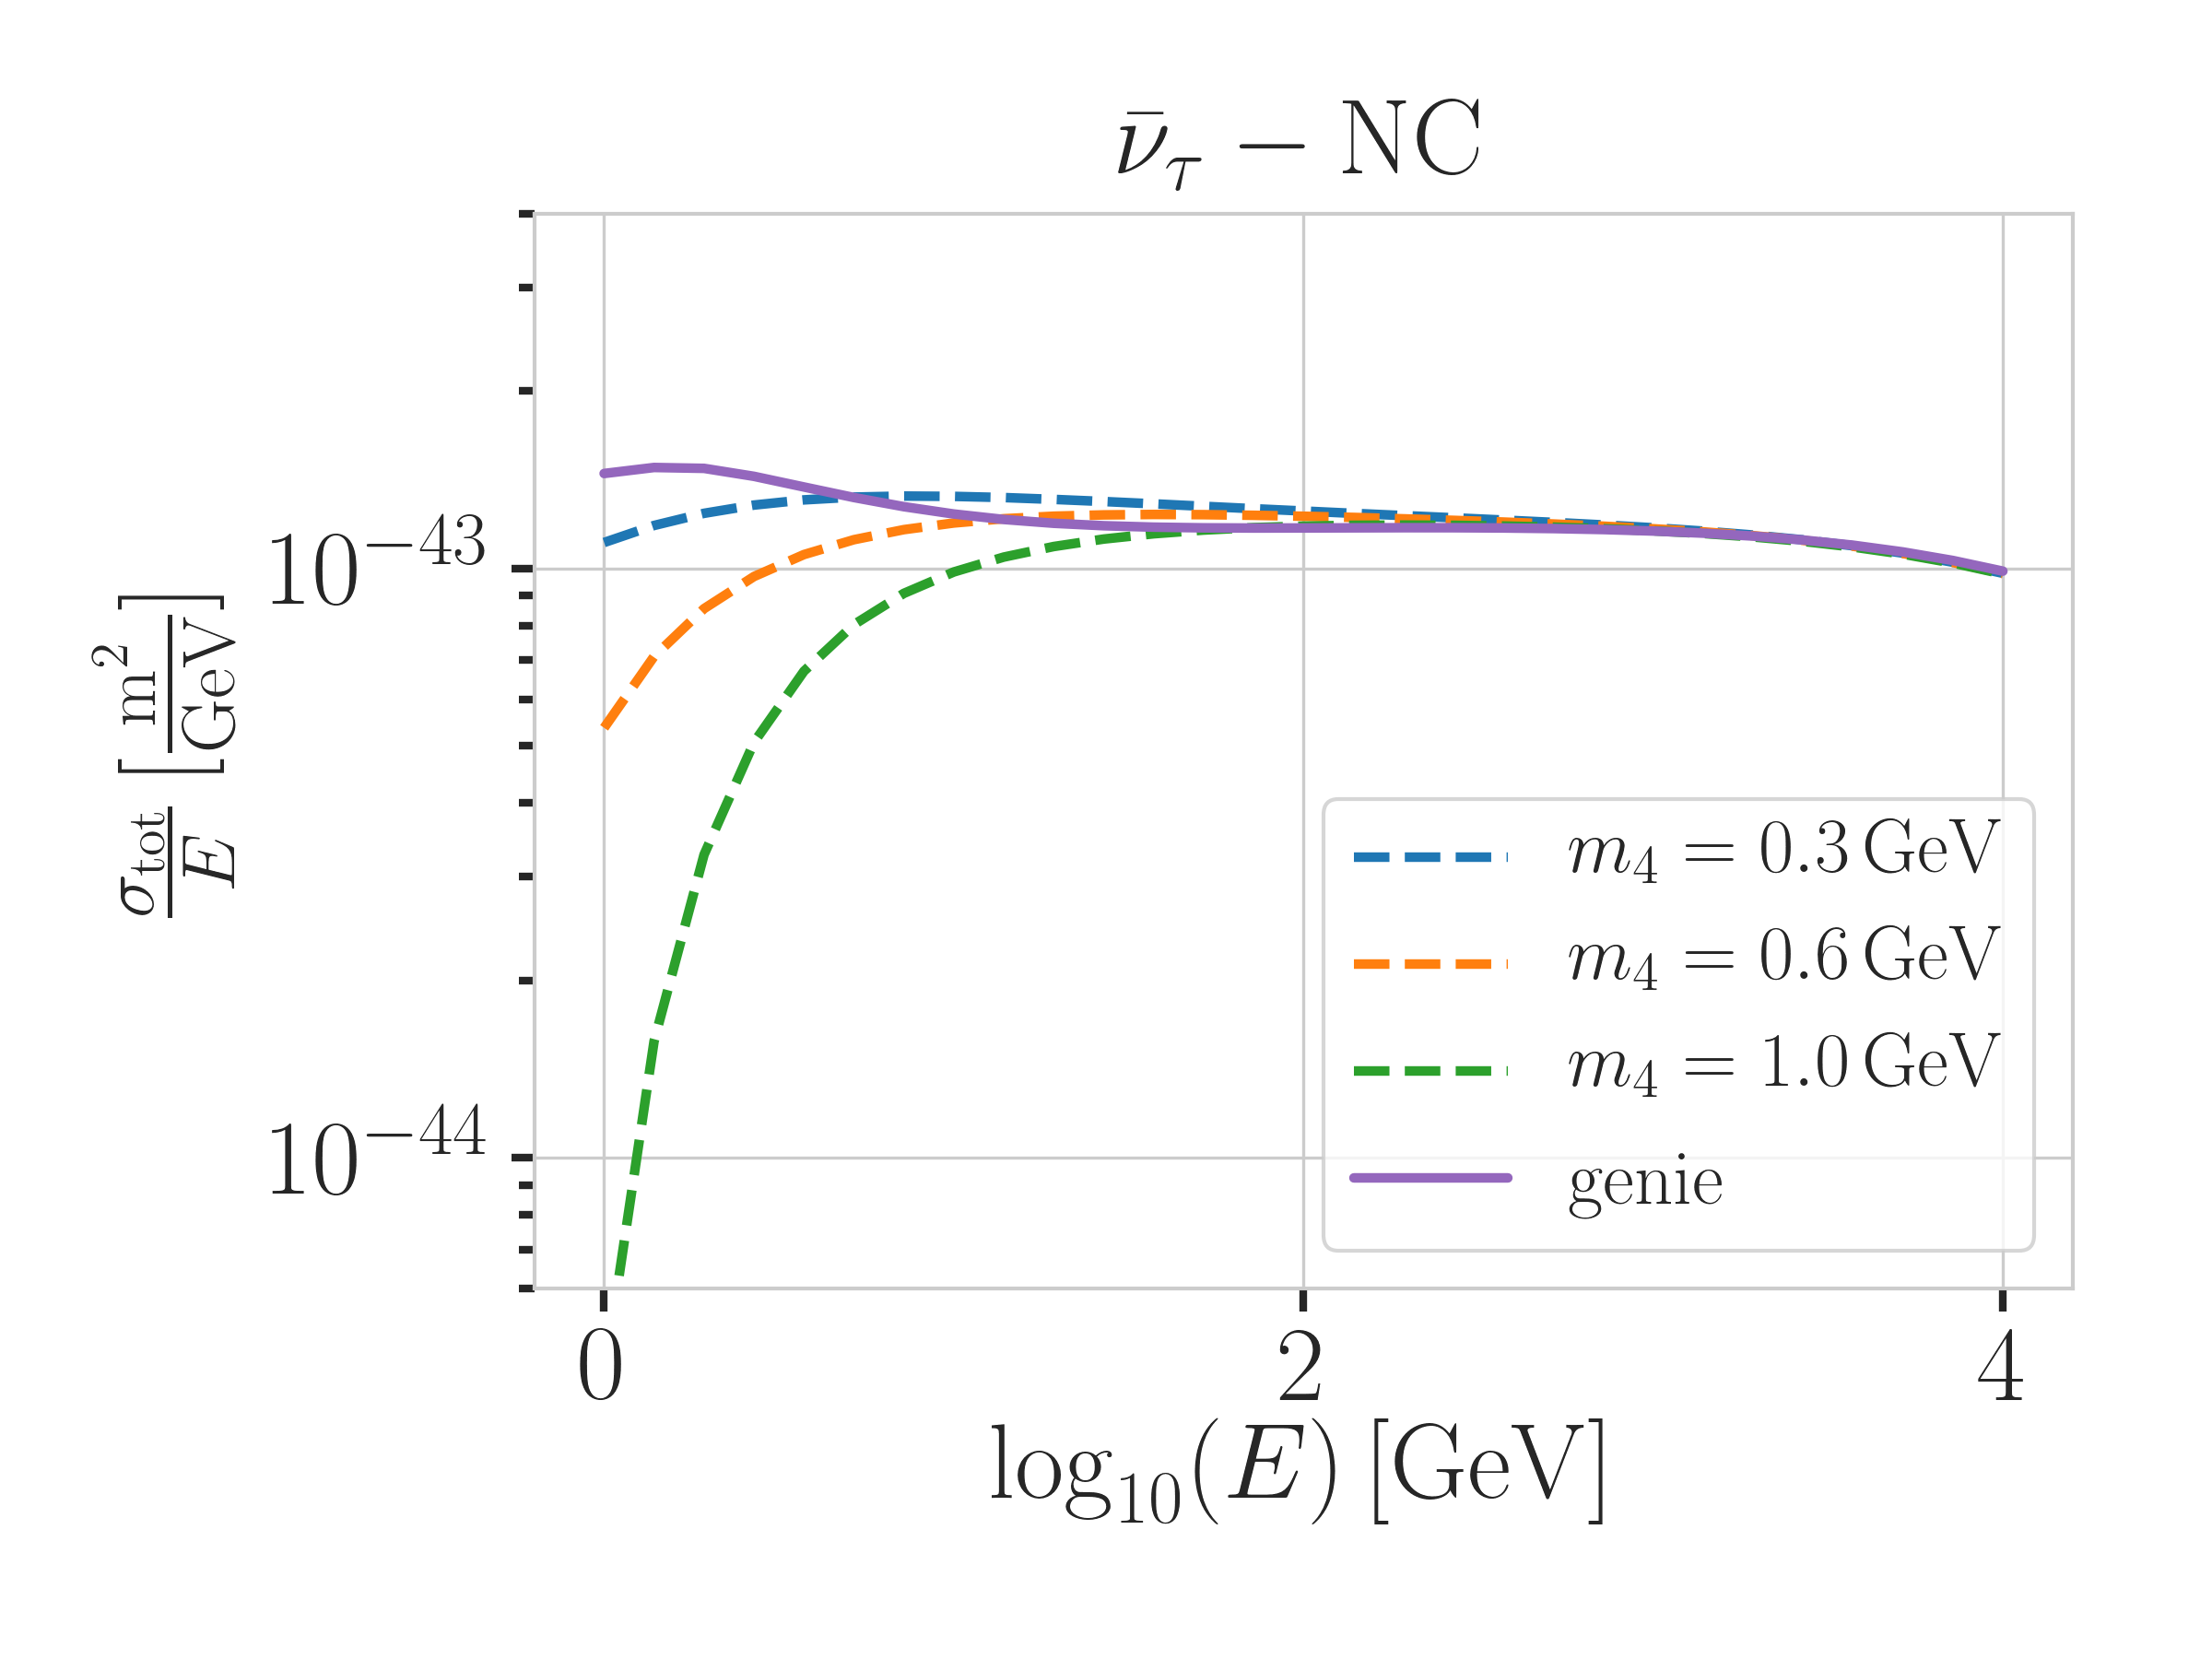
\includegraphics[width=.49\linewidth]{figures/hnl_simulation/cross_sections/custom_HNL_thesis_sigma-nutaubar-N-nc.png}
    \caption
    [Custom HNL total cross-sections]{Custom HNL total cross-sections for the three target masses compared to the total ($\nu_\tau$/$\bar{\nu}_\tau$ NC) cross-sections used for SM neutrino simulation production with GENIE.}
    \labfig{custom_hnl_cross_sections}
\end{figure*}

The GRV98LO PDFs were added to the cross-section spline maker and used to create the HNL cross-sections for consistency with the neutrino simulation explained in \refsec{neutrino_generation}. The double-differential ($\rm{d}^2\sigma/\rm{d}x\rm{d}y$) and total ($\sigma$) cross-sections were produced for the chosen target HNL masses and then splined in energy, $x$, and $y$ for $\rm{d}^2\sigma/\rm{d}x\rm{d}y$ and $\sigma$ in the energy. \reffig{custom_hnl_cross_sections} shows the total cross-sections that were produced compared to the cross-section used for the production of the SM $\nu_\tau/\bar{\nu}_\tau$ NC background simulation. They agree above $\sim\SI{200}{\GeV}$, where the modification should not have any effect on the cross-sections. This is the desired result of using the identical input PDFs, and confirms that the unmodified cross-sections produced with NuXSSplMkr agree with the GENIE cross-sections.


\subsubsection{Decay Channels}

The accessible decay channels are dependent on the mass of the HNL and the allowed mixing. For this analysis, where only $|U_{\tau4}|^2 \neq 0$, the decay channels considered are listed in \reftab{hnl_decay_channels} and the corresponding branching ratios are shown in \reffig{hnl_branching_ratios}. The individual branching ratio for a specific mass is calculated as $\mathrm{BR}_i(m_4)=\Gamma_i(m_4)/\Gamma_\mathrm{total}(m_4)$, where $\Gamma_\mathrm{total}(m_4)=\sum\Gamma_i(m_4)$. The individual decay widths $\Gamma_i$ are computed using the state-of-the-art calculations from \sidecite{Coloma:2020lgy}, which are described in the following.

\begin{margintable}
    % \footnotesize
    \begin{tabular} { lr }
        \hline\hline 
        \textbf{Channel} & \textbf{Opens}  \\
        \hline\hline 
        $\nu_4 \rightarrow \nu_\tau \nu_\alpha \bar{\nu_\alpha}$ & \SI{0}{\MeV} \\
        $\nu_4 \rightarrow \nu_\tau e^+ e^-$ & \SI{1}{\MeV} \\
        $\nu_4 \rightarrow \nu_\tau \pi^0$ & \SI{135}{\MeV} \\
        $\nu_4 \rightarrow \nu_\tau \mu^+ \mu^-$ & \SI{211}{\MeV} \\
        $\nu_4 \rightarrow \nu_\tau \eta$ & \SI{548}{\MeV} \\
        $\nu_4 \rightarrow \nu_\tau \rho^0$ & \SI{770}{\MeV} \\
        $\nu_4 \rightarrow \nu_\tau \omega$ & \SI{783}{\MeV} \\
        $\nu_4 \rightarrow \nu_\tau \eta'$ & \SI{958}{\MeV} \\
        \hline
    \end{tabular}
    \caption[HNL mass dependent decay channels]{Possible decay channels of the HNL, considering only $|U_{\tau4}|^2 \neq 0$, and the mass at which each channel opens.}
    \labtab{hnl_decay_channels}
\end{margintable}

\begin{figure}[h]
    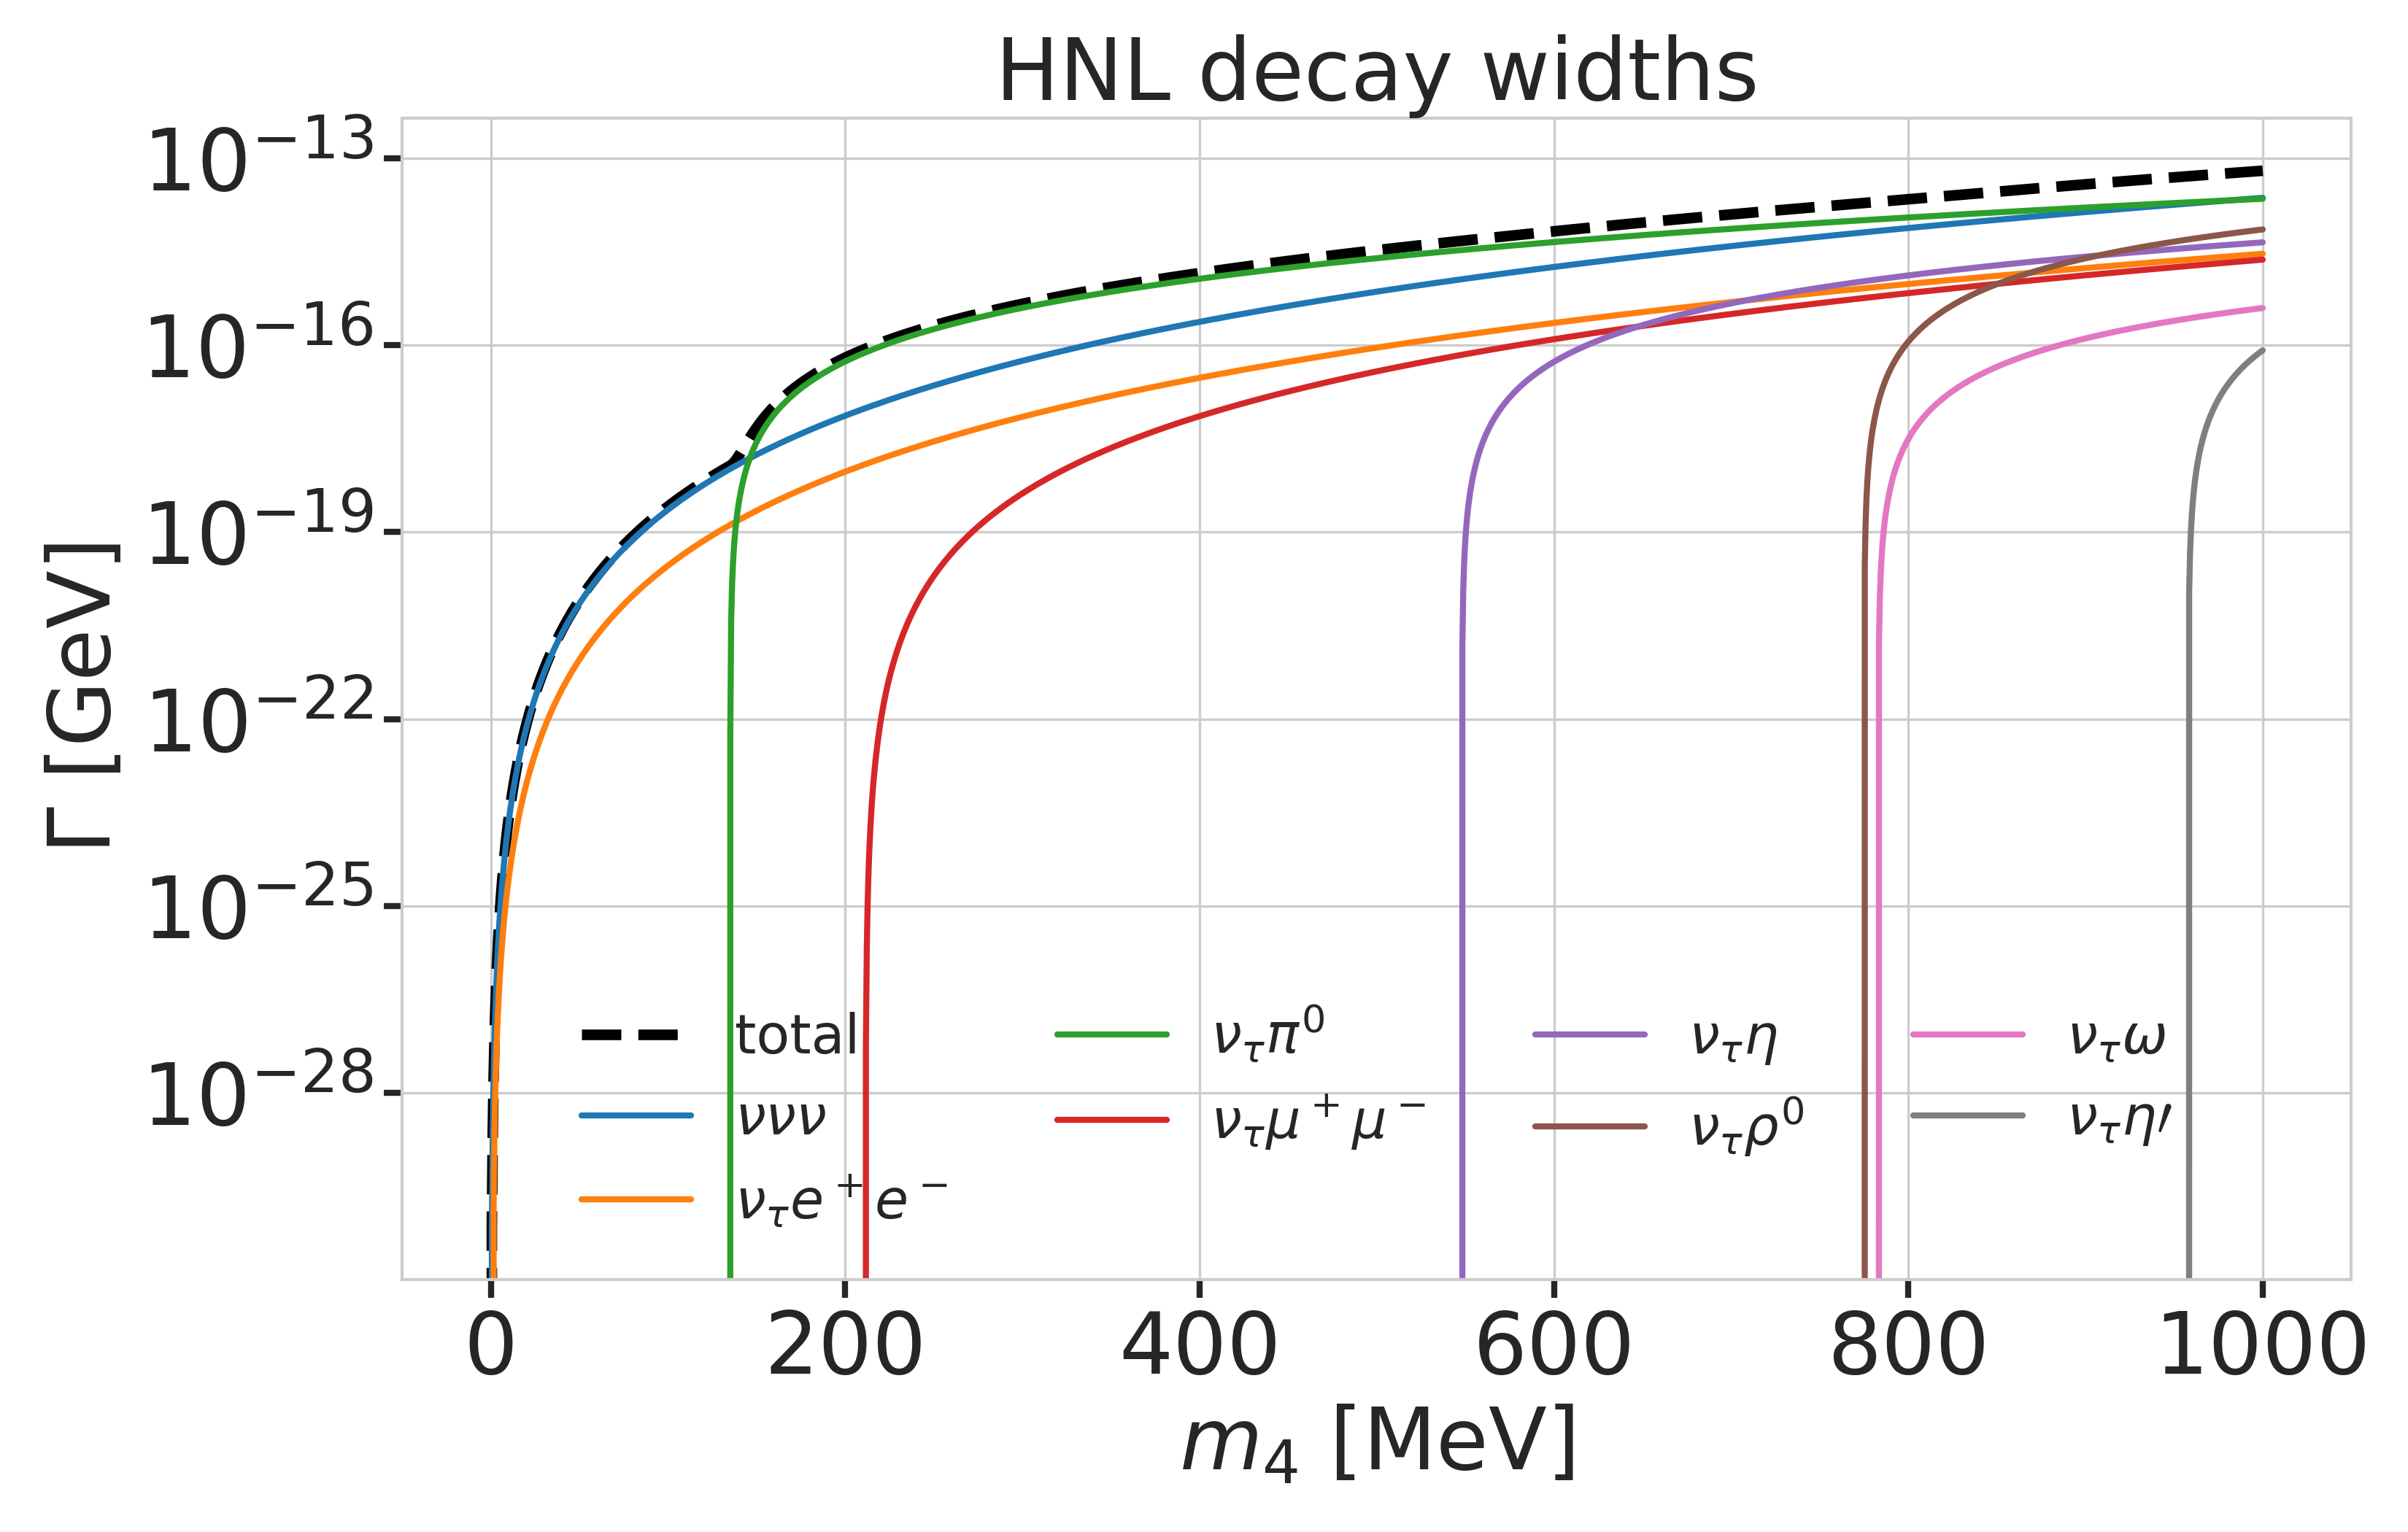
\includegraphics{figures/hnl_simulation/decay_theory/hnl_decay_widths_up_to_1.0_GeV_linear.png}
    \caption[HNL decay widths]{Decay widths of the HNL within the mass range considered, calculated based on the results from \cite{Coloma:2020lgy}. Given the existing constraints on $|U_{e4}|^{2}$ and $|U_{\mu4}|^{2}$, we consider that the corresponding decay modes are negligible.}
    \labfig{hnl_decay_modes_log_decay_width}
\end{figure}
\todo{say something about the decay widht plot, mention it in the text.. (RED)}


\paragraph{2-Body Decay Widths}

The decay to a neutral pseudoscalar meson is
\begin{equation}
    \Gamma_{\nu_4 \rightarrow \nu_\tau P} = |U_{\tau4}|^2 \frac{G_F^2 m_4^3}{32\pi} f_P^2 (1-x_p^2)^2
    \;,
    \labeq{gamma_nu_P}
\end{equation}
with $x_P = m_P/m_4$ and the \textit{effective decay constants $f_P$} given by
\begin{align}
    f_{\pi^0} ={}& +\SI{0.1300}{\GeV}\;, \\
    f_{\eta} ={}& +\SI{0.0816}{\GeV}\;, \rm{and} \\
    f_{\eta'} ={}& -\SI{0.0946}{\GeV}\;,
    \labeq{gamma_nu_P_f_factors}
\end{align}
while the decay to a neutral vector meson is given by
\begin{equation}
    \Gamma_{\nu_4 \rightarrow \nu_\tau V} = |U_{\tau4}|^2 \frac{G_F^2 m_4^3}{32\pi} \bigg(\frac{f_V}{m_V}\bigg)^2 g_V^2 (1+2x_V^2) (1-x_V^2)^2
    \;,
    \labeq{gamma_nu_V}
\end{equation}
with $x_V = m_V/m_4$,
\begin{align}
    f_{\rho^0} ={}& \SI{0.171}{\square\GeV}\;, \\
    f_{\omega} ={}& \SI{0.155}{\square\GeV}\;,
    \labeq{gamma_nu_V_f_factors}
\end{align}
and
\begin{align}
    g_{\rho^0} ={}& 1-2\sin^2{\theta_w}\;, \\
    g_{\omega} ={}& \frac{-2\sin^2{\theta_w}}{3}\;,
    \labeq{gamma_nu_V_g_factors}
\end{align}
and $\sin^2{\theta_w}=0.2229$ \sidecite{codata2018}, where $\theta_w$ is the Weinberg angle.


\paragraph{3-Body Decay Widths}

The (invisible) decay to three neutrinos, one of flavor $\tau$ and two of any flavor $\alpha$, is
\begin{equation}
    \Gamma_{\nu_4 \rightarrow \nu_\tau \nu_\alpha \bar{\nu_\alpha}} = |U_{\tau4}|^2 \frac{G_F^2 m_4^5}{192\pi^3}
    \;,
    \labeq{gamma_nu_nu_nu}
\end{equation}
while the decay to two charged leptons (using $x_\alpha = (m_\alpha/m_4)^2)$ of the same flavor reads
\begin{equation}
    \Gamma_{\nu_4 \rightarrow \nu_\tau l_\alpha^+ l_\alpha^-} = |U_{\tau4}|^2 \frac{G_F^2 m_4^5}{192\pi^3} \big[ C_1 f_1(x_\alpha) + C_2 f_2(x_\alpha) \big]
    \;,
    \labeq{gamma_nu_ll_full}
\end{equation}
with the constants defined as
\begin{align}
    C_1 ={}& \frac{1}{4}(1-4\sin^2{\theta_w}+8\sin^4{\theta_w})\;, \\
    C_2 ={}& \frac{1}{2}(-\sin^2{\theta_w}+2\sin^4{\theta_w})\;,
    \labeq{gamma_nu_ll_c1_c2}
\end{align} 
the functions as
\begin{equation}
    f_1(x_\alpha) = (1-14x_\alpha-2x_\alpha^2-12x_\alpha^3)\sqrt{1-4x_\alpha}+12x_\alpha^2(x_\alpha^2-1)L(x_\alpha)
    \;,
    \labeq{gamma_nu_ll_f1}
\end{equation}
\begin{equation}
    f_2(x_\alpha) = 4[x_\alpha(2+10x_\alpha-12x_\alpha^2)\sqrt{1-4x_\alpha}+6x_\alpha^2(1-2x_\alpha+2x_\alpha^2)L(x_\alpha)]
    \;,
    \labeq{gamma_nu_ll_f2}
\end{equation}
and
\begin{equation}
    L(x) = \ln \biggl( \frac{ 1-3x_\alpha-(1-x_\alpha)\sqrt{1-4x_\alpha} }{ x_\alpha(1+\sqrt{1-4x_\alpha}) } \biggr)
    \;.
    \labeq{gamma_nu_ll_l}
\end{equation}


\subsubsection{Analytical 2-Body Decay Kinematics}

Following the review of \sidecite{PDG_review_2022}, the 4-vector defining the kinematics of a particle is $p=(E,\vec{p})$, with its energy, $E$, and 3-momentum, $\vec{p}$. Squaring it gives the mass, $p^2=E^2-\vec{p}^2=m^2$, while the velocity is $\vec{\beta}=\vec{p}/E$. If the HNL with mass $m_4$ decays into two particles with masses $m_1$ and $m_2$, their 3-momenta in the rest frame of the HNL are given by
\begin{equation}
    |\vec{p}_1| = |\vec{p}_2| = \frac{\lambda^{1/2}(m_4^2,m_1^2,m_2^2)}{2m_4}
    \;,
    \labeq{2body_momenta}
\end{equation}
where $\lambda(x,y,z)=x^2+y^2+z^2-2xy-2xz-2yz$. The energy of the particles is then given by
\begin{equation}
    E_1 = \frac{m_4^2+m_1^2-m_2^2}{2m_4}
    \;,
    \labeq{2body_energies}
\end{equation}
and equivalently for $E_2$. The 4-vectors of the particle are then boosted to the lab frame, where the HNL is moving with velocity $\vec{\beta}$.


\subsubsection{Simulated 3-Body Decay Kinematics}

The 3-body decay kinematics cannot be computed analytically, instead, we employ \textsc{MadGraph4} (v3.4.0) \cite{madgraph4} for this purpose. MadGraph is a tool to simulate particle collisions and decay processes, and is widely used in the high-energy physics community. The 3-body decay kinematics are calculated in the rest frame of the HNL, using decay diagrams calculated with \textsc{FeynRules 2.0} \sidecite{feynrules2} and the Lagrangians derived in \sidecite{Coloma:2020lgy} as input. The \textit{Universal FeynRules Output (UFO)} from \textsc{effective\_HeavyN\_Majorana\_v103} were used for our calculation. For each mass and corresponding decay channels, we produce \SI{1e06} decay kinematic variations in the rest frame and store those in a text file. During event generation, we uniformly select an event from that list, to simulate the decay kinematics of a 3-body decay.


\subsection{Sampling Distributions} \labsec{hnl_sampling_distributions}

\begin{table}[H]
    \centering
    \begin{tabular} { lll }
        \hline \hline 
        \textbf{Variable} & \textbf{Distribution} & \textbf{Range/Value} \\
        \hline \hline 
        energy & $E^{-2}$ & [\SI{2}{\GeV}, \SI{1e4}{\GeV}] \\
        zenith & uniform (in $\cos(\theta)$) & [\SI{80}{\degree}, \SI{180}{\degree}] \\
        azimuth & uniform & [\SI{0}{\degree}, \SI{360}{\degree}] \\
        vertex $x,y$ & uniform (on circle) & $r$=\SI{600}{\metre} \\
        vertex $z$ & uniform & \SIrange{-600}{0}{\metre} \\
        $m_\mathrm{4}$ & fixed & [0.3, 0.6, 1.0]\,\si{\GeV} \\
        $L_\mathrm{decay}$ & $L^{-1}$ & [0.0004, 1000]\,\si{\metre} \\
        \hline
    \end{tabular}
    \caption[Model-dependent simulation sampling distributions]{Generation level sampling distributions and ranges/values of the model-dependent simulation samples.}
    \labtab{model_dendent_sample_sampling_distributions}
\end{table}

In principle, the generation level sampling distributions should be chosen such that at the final level of the event selection chain the phase space relevant for the analysis is covered with sufficient statistics to make a reasonable estimate of the event expectation. Initial distributions insufficiently covering the phase space lead to an underestimation of the expected rates, because some of the events that would pass the selection are not produced. This limits the expected analysis potential. Three discrete simulation samples were produced with HNL masses of \SI{0.3}{\GeV}, \SI{0.6}{\GeV}, and \SI{1.0}{\GeV}. The remaining sampling distributions are identical for all samples and are listed in \reftab{model_dendent_sample_sampling_distributions}. The target number of events for each sample was \SI{2.5e9}{} at generation to result in sufficient MC statistics at final level. \reffig{hnl_gen_distris} shows the true cascade energies, which result from the custom interaction cross-sections and the decays discussed above. Note here that these are the full true energies going into the cascades. For the first cascade some energy goes into invisible particles produced in the hadronic shower development and for the HNL decay, there always is at least one invisible neutrino. Additional sampling distributions can be found in \reffig{hnl_gen_distris_appendix}.
\begin{figure*}[h]
    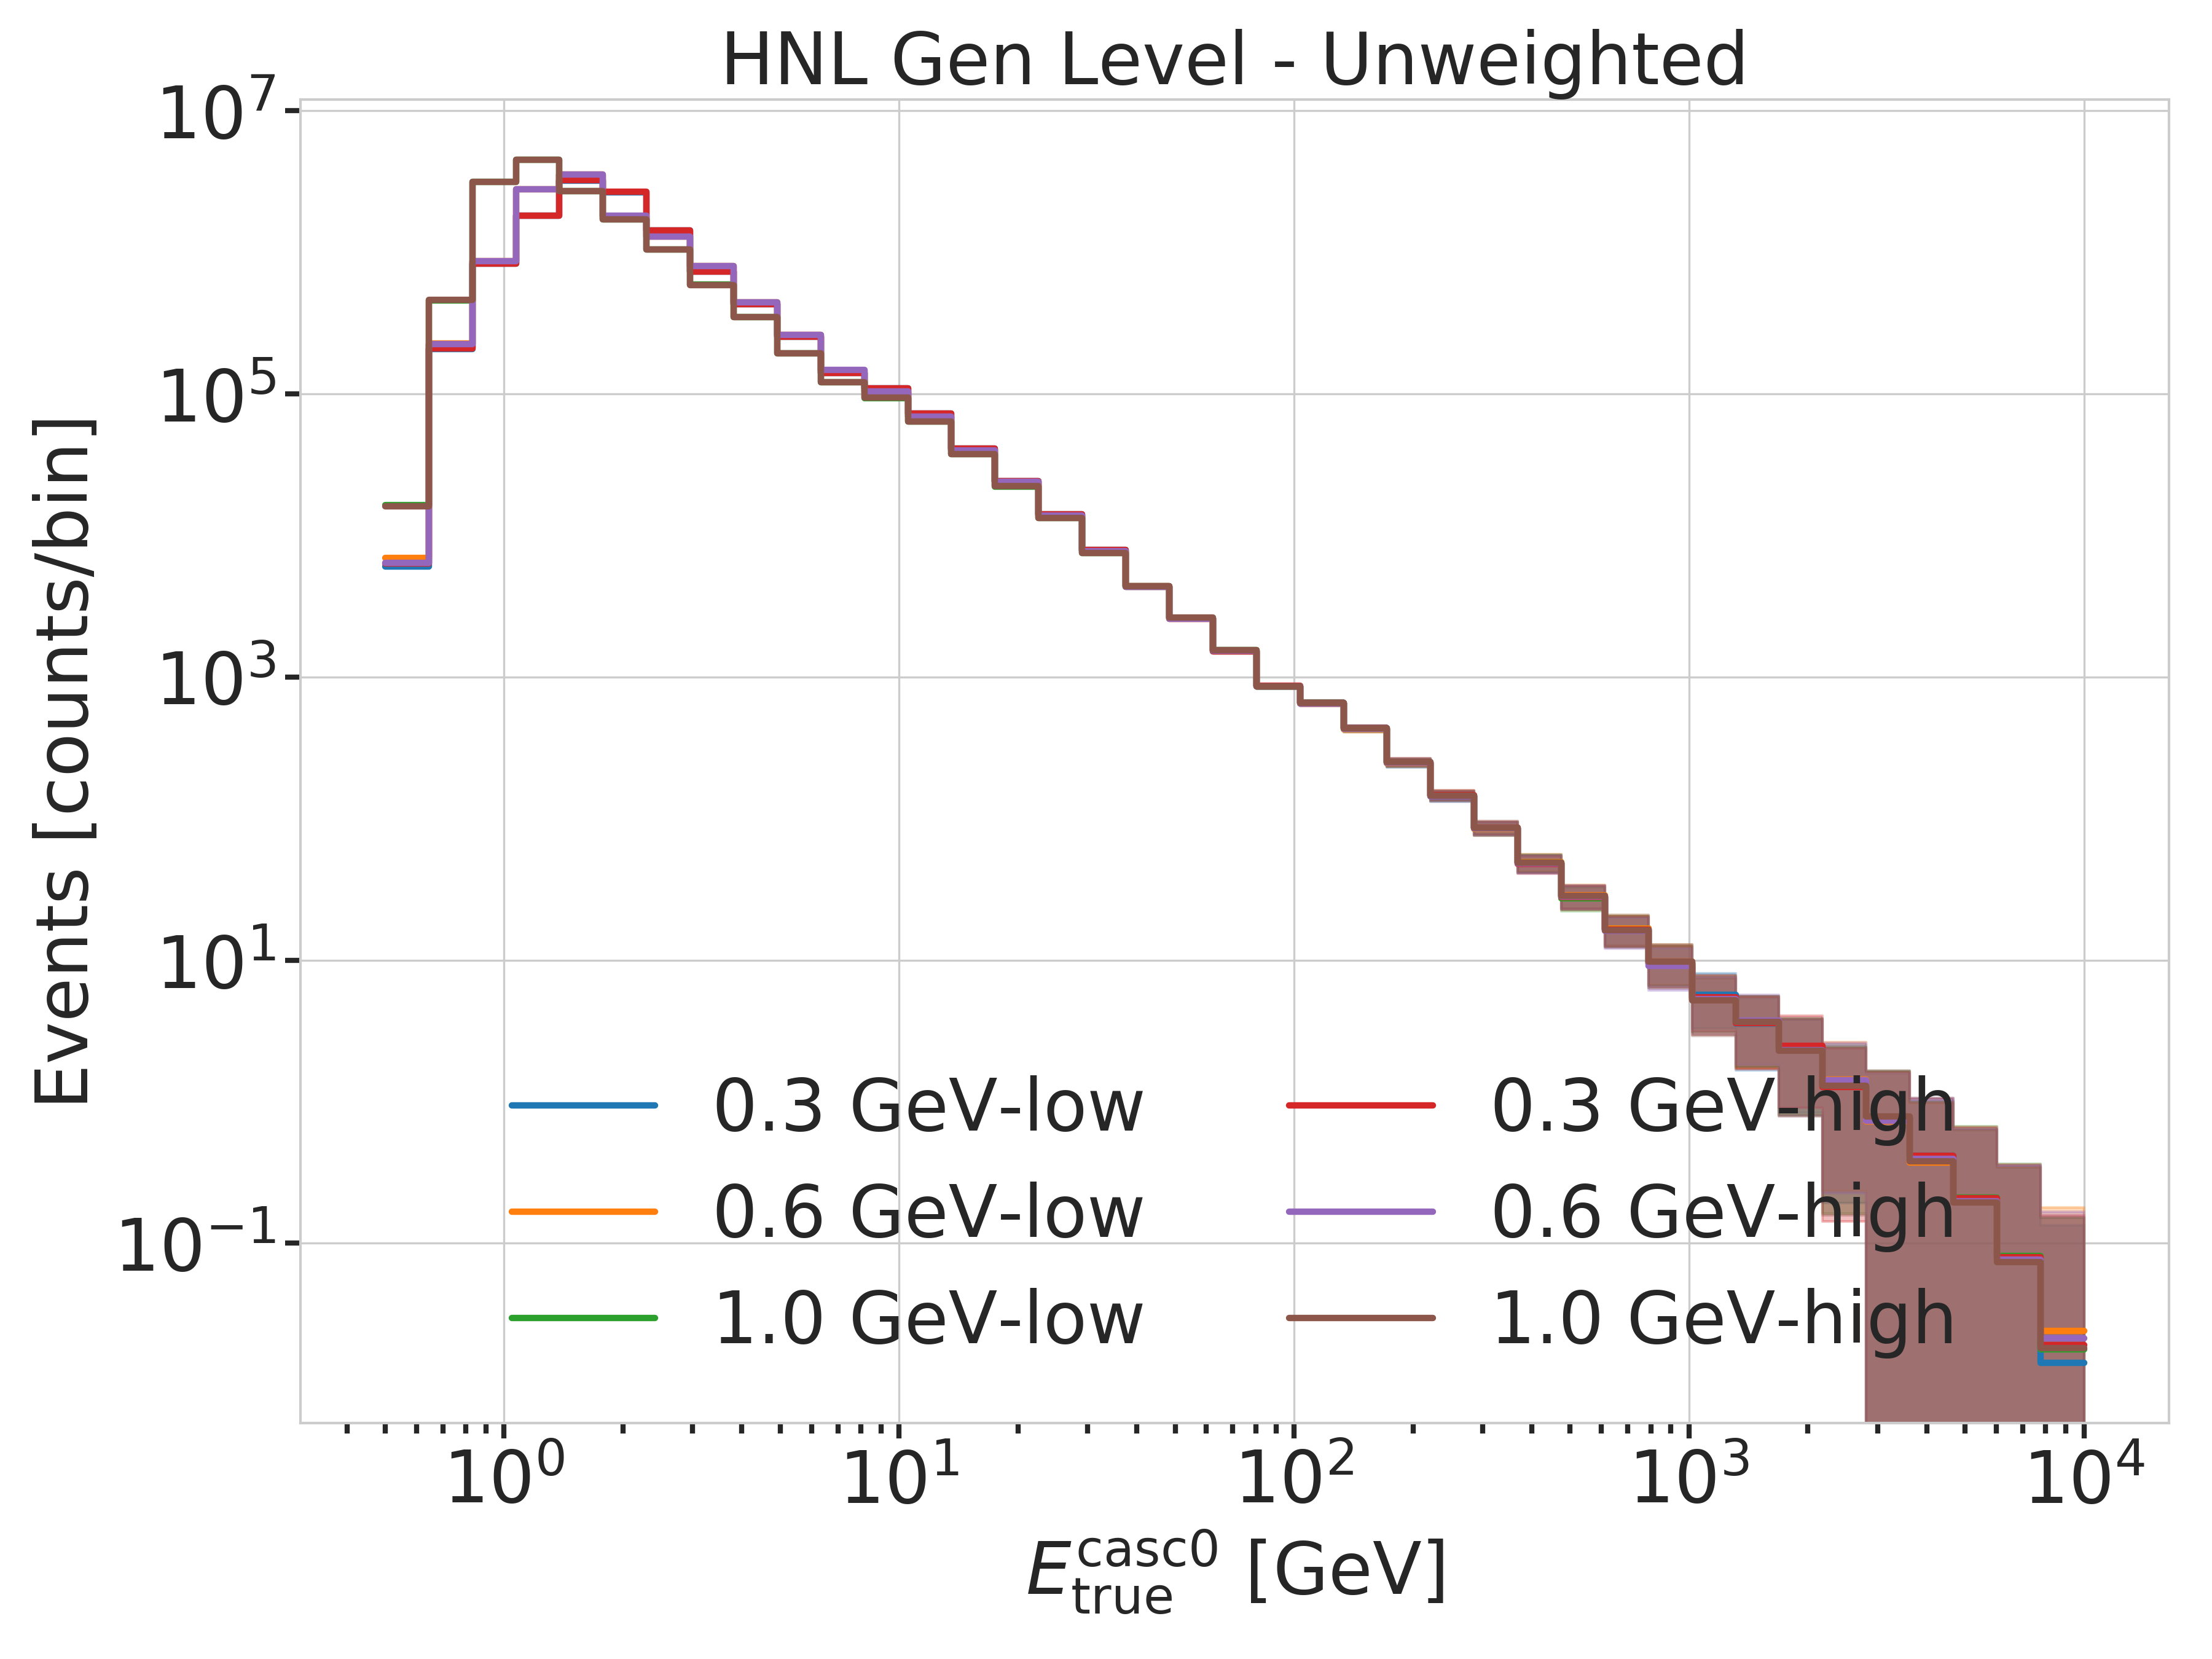
\includegraphics[width=0.49\linewidth]{figures/hnl_simulation/generation/1_d_distr_casc0_true_energy_gen_level_unweighted.png}
    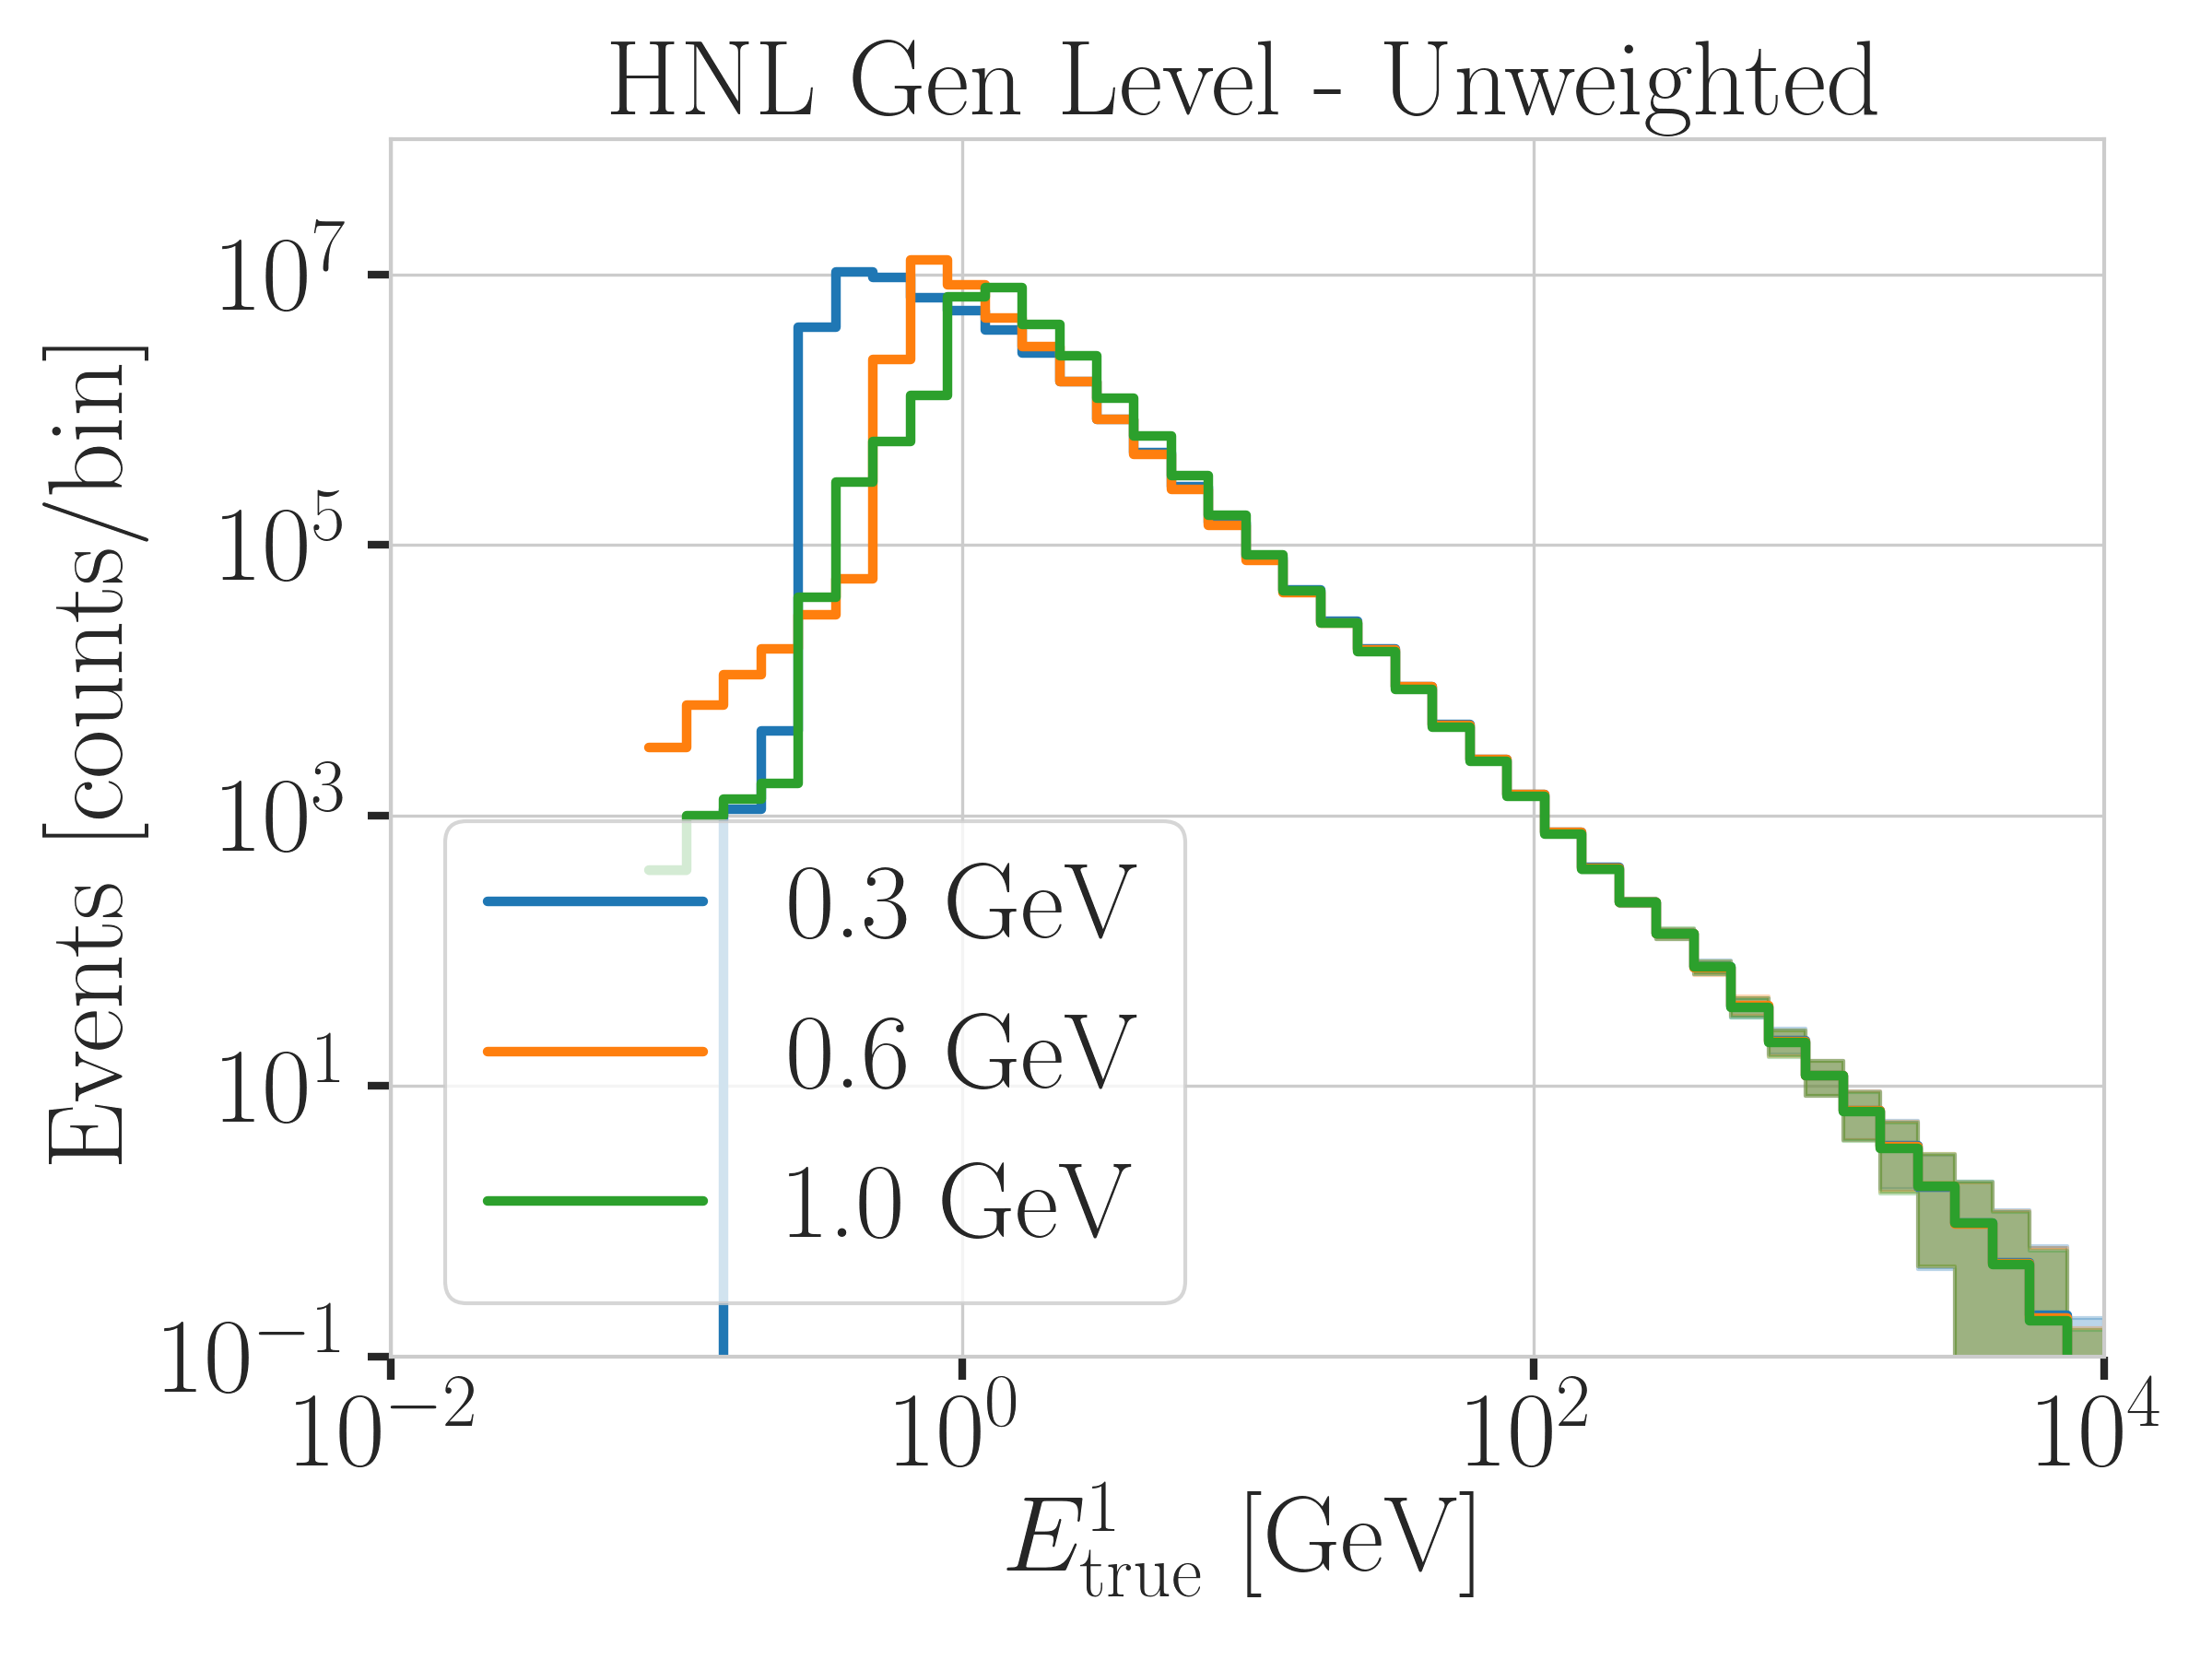
\includegraphics[width=0.49\linewidth]{figures/hnl_simulation/generation/1_d_distr_casc1_true_energy_gen_level_unweighted.png}
    \caption[Model-dependent simulation generation level distributions]{Generation level distributions of the model-dependent simulation. Shown are the true energies of both cascades including the energy that goes into invisible particles.}
    \labfig{hnl_gen_distris}
\end{figure*}


\subsection{Weighting Scheme} \labsec{hnl_weighting_scheme}

\todo{JVS:
    The build-up of the weight expression is hard to follow without knowing where it’s going. It may be better to start with the fact that the importance sampling weight is the ratio of PDFs, then write down each pdf, then drill down into each of the terms (basically, the standard “tell me what you’re going to tell me, then tell me, then tell me what you told me” scheme). (RED)
}

To produce physically correct event distributions based on the simplified generation sampling distributions, each event has to be re-weighted. The only required input is the mixing strength $|U_{\tau4}|^2$, which is the variable physics parameter in this analysis. For each event the gamma factor
\begin{equation}
    \gamma = \frac{\sqrt{E_\mathrm{kin}^2+m_4^2}}{m_4}
    \;,
    \labeq{gamma_factor}
\end{equation}
is calculated, with the HNL mass $m_4$, and its kinetic energy $E_\mathrm{kin}$. The speed of the HNL is calculated as
\begin{equation}
    v = c \cdot \sqrt{1 - \frac{1}{\gamma^2}}
    \;,
    \labeq{lorentz_speed}
\end{equation}
where $c$ is the speed of light. With these, the lab frame decay length range $[s_\mathrm{min},s_\mathrm{max}]$ can be converted into the rest frame lifetime range $[\tau_\mathrm{min},\tau_\mathrm{max}]$ for each event
\begin{equation}
    \tau_\mathrm{min/max} = \frac{s_\mathrm{min/max}}{v\cdot\gamma}.
\end{equation}
The proper lifetime of each HNL event can be calculated using the total decay width $\Gamma_\mathrm{total}$ from \refsec{custom_leptoninjector} and the chosen mixing strength $|U_{\tau4}|^2$ as
\begin{equation}
    \tau_\mathrm{proper} = \frac{\hbar}{\Gamma_\mathrm{total}(m_4) \cdot |U_{\tau4}|^2}
    \;,
    \labeq{proper_lifetime}
\end{equation}
where $\hbar$ is the reduced Planck constant. Since the decay lengths or lifetimes of the events are sampled from an inverse distribution instead of an exponential, as it would be expected from a particle decay, we have to re-weight accordingly to achieve the correct decay lengths or lifetimes distribution. This is done by using the desired exponential distribution
\begin{equation}
    \mathrm{PDF}_\mathrm{exp} = \frac{1}{\tau_\mathrm{proper}} \cdot e^{\frac{-\tau}{\tau_\mathrm{proper}}}
    \;,
    \labeq{pdf_exponential}
\end{equation}
and the inverse distribution that was sampled from
\begin{equation}
    \mathrm{PDF}_\mathrm{inv} = \frac{1}{\tau \cdot (\ln(\tau_\mathrm{max}) - \ln(\tau_\mathrm{min}))}
    \;.
    \labeq{pdf_inverse}
\end{equation}
This re-weighting factor is then calculated as
\begin{equation}
    w_\mathrm{lifetime} = \frac{\mathrm{PDF}_\mathrm{exp}}{\mathrm{PDF}_\mathrm{inv}} = \frac{\Gamma_\mathrm{total}(m_4) \cdot |U_{\tau4}|^2}{\hbar} \cdot \tau \cdot (\ln(\tau_\mathrm{max}) - \ln(\tau_\mathrm{min})) \cdot e^{\frac{-\tau}{\tau_\mathrm{proper}}}
    \;.
    \labeq{weight_lifetime}
\end{equation}
Adding another factor of $|U_{\tau4}|^2$ to account for the mixing at the interaction vertex the total re-weighting factor becomes
\begin{equation}
    w_\mathrm{total} = |U_{\tau4}|^2 \cdot w_\mathrm{lifetime}
    \;.
    \labeq{weight_full}
\end{equation}
If this additional weighting factor is multiplied to the generation weight from \refeq{neutrino_generation_weight} with units \si{\meter^2}, the livetime in \si{\second}, and the oscillated primary neutrino flux in \si{\meter^{-2}\second^{-1}}, it results in the number of expected events in the detector for this particular MC event for a chosen mixing (and mass).


\section{Standard Model Event Generation} \labsec{sm_event_generation}


\subsection{Neutrinos} \labsec{neutrino_generation}

The simulation volume is a cylinder centered in DeepCore with radius and height chosen such that all events possibly producing a signal are contained. The different sizes, chosen depending on energy and neutrino flavor, are shown in \reftab{genie_sampling_cylinder}.
\begin{table}
    \begin{center}
        \footnotesize
        \begin{tabular}{ l l l l l l }

            \hline\hline

            \textbf{Flavor} & \textbf{Energy [\si{\gev}]} & \textbf{Radius [\si{\metre}]} & \textbf{Length [\si{\metre}]} & \textbf{Events/File}  & \textbf{Files}\\ 

            \hline\hline

            \multirow{4}{*}[-1.em]{ $\nu_e+\bar{\nu_e}$ }
            & 1-4
            & \multirow{1}{*}[-1.em]{ 250 }
            & \multirow{1}{*}[-1.em]{ 500 }
            & 450000
            & \multirow{4}{*}[-1.em] {650} \\

            \cmidrule{2-2}
            \cmidrule{5-5}
            
            & 4-12
            & 
            & 
            & \multirow{1}{*}[-1.em] { 100000 }
            & \\

            \cmidrule{2-4}

            & 12-100
            & 350
            & 600
            & 
            & \\

            \cmidrule{2-5}

            & 100-10000
            & 550
            & 1000
            & 57500
            & \\

            \hline
            \hline

            \multirow{4}{*}[-1.em]{ $\nu_\mu+\bar{\nu_\mu}$ }
            & 1-5
            & 250
            & 500
            & 408000
            & \multirow{4}{*}[-1.em] {1550} \\

            \cmidrule{2-5}
            
            & 5-80
            & 400
            & 900
            & 440000
            & \\

            \cmidrule{2-5}

            & 80-1000
            & 450
            & \multirow{1}{*}[-1.em] { 1500 }
            & 57500
            & \\

            \cmidrule{2-3}
            \cmidrule{5-5}

            & 1000-10000
            & 550
            &
            & 6700
            & \\

            \hline
            \hline

            \multirow{4}{*}[-1.em]{ $\nu_\tau+\bar{\nu_\tau}$ }
            & 1-4
            & \multirow{1}{*}[-1.em]{ 250 }
            & \multirow{1}{*}[-1.em]{ 500 }
            & 1500000
            & \multirow{4}{*}[-1.75em] {350} \\

            \cmidrule{2-2}
            \cmidrule{5-5}
            
            & 4-10
            & 
            & 
            & 300000
            & \\

            \cmidrule{2-5}

            & 10-50
            & 350
            & 600
            & 375000
            & \\

            \cmidrule{2-5}

            & 50-1000
            & 450
            & 800
            & 200000
            & \\

            \cmidrule{2-5}

            & 1000-10000
            & 550
            & 1500
            & 26000
            & \\

            \hline

        \end{tabular}
    \end{center}
    \caption[GENIE generation cylinder volumes]{Cylinder volumes used for GENIE neutrino simulation generation. Cylinder is always centered in DeepCore at $(x,y,z) = (46.29,-34.88,-330.00)$ \si{\metre}.}\labtab{genie_sampling_cylinder}
\end{table}
The directions of the neutrinos are sampled isotropically and the energies are sampled from an $E^{-2}$ power law. The number of simulated events is chosen such that the livetime is more than \SI{70}{years} for each flavor. Neutrinos and antineutrinos are simulated with ratios of 70\% and 30\%, respectively, which is roughly the ratio expected from the atmospheric neutrino flux \sidecite{PhysRevD.92.023004_Honda_Flux}.

To simulate the neutrino interaction with the ice, the \textsc{Genie} event generator \sidecite{genie} (version 2.12.8) is used, resulting in the secondary particles and the kinematic and cross-section parameters. As input, the outdated \href{https://internal.dunescience.org/doxygen/classgenie_1_1GRV89LO.html}{GRV98LO} \sidecite{grv98_pdf} PDFs were used, because they were the only option that could incorporate extrapolations to lower $Q^2$ \sidecite{grv98_effective_low_q2}. The propagation of the secondary particles and of the shower development is performed identical to the description in \refsec{custom_leptoninjector} and produces the energy losses and event morphologies introduced in \refsec{icecube_propagation}.


\subsection{Muons}

Atmospheric muons are generated on a cylinder surface enclosing the full IceCube detector array. The cylinder has a height of \SI{1600}{\meter} and a radius of \SI{800}{\meter}. The energy is sampled from an $E^{-3}$ power law while the other sampling distributions (position, direction) are found from parameterizations based on \sidecite{muon_parameterization}. This work uses full \textsc{Corsika} \sidecite{corsika} simulations of muons to tailor the parameterizations, starting from \textit{cosmic ray (CR)} interactions with atmospheric nuclei using the CR flux model from \sidecite{gaisser_cosmic_ray} and producing the muons applying the hadronic interaction model SIBYLL 2.1 \sidecite{sibyll_hadronic}. After the generation, they are propagated through the ice with PROPOSAL producing photons, treating them exactly like the muons produced in the HNL and neutrino event generation.

Since the offline processing and selection steps described in \refsec{event_selection} and \refsec{reconstruction} reduce the muon contamination to an almost negligible level, the statistical uncertainty on the number of expected muon events at the final selection level is large and therefore two separate samples of muon simulation are produced. \textbf{A first sample} is used to tune the lower level selection (up to Level 4), therefore including all events resulting from the above described generation. \textbf{A second sample} is then produced to estimate the muon contamination at higher levels (above Level 5). It only consists of muon events that pass through a smaller cylinder centered in DeepCore (height of \SI{400}{\meter} and radius of \SI{180}{\meter}), and additionally rejects events based on a KDE estimated muon density at Level 5 (in energy and zenith). This increased the simulation efficiency at Level 5 significantly, making it feasable to use this sample to estimate the muon contamination at higher levels.


\section{Detector Simulation} \labsec{detector_simulation}

The detector simulation is performed after the event generation, where the initial particles and the resulting photons and secondary particles from their propagation were produced. This part of the simulation chain is applied to all muon and neutrino simulation as well as the HNL signal simulation explained in detail in \refch{signal_simulation}. The detector simulation can be split into two parts: the propagation of the photons and the simulation of the detector response (including internal noise).


\subsection{Photon Propagation} \labsec{photon_propagation}

% For any Cherenkov detector, but especially for ice-Cherenkov detectors, like IceCube, the propagation of the photons is a crucial part of the detector simulation.
Any photon that was produced in the event generation is individually traced through the ice, simulating scattering and absorption processes.
% , taking into account the local ice properties, estimated with a chosen ice model.
The propagation is done using \textsc{clsim} \cite{clsim} which is an implementation of the \textit{Photon Propagation Code (\textsc{PPC})} \sidecite{ppc} in \textsc{OpenCL}. It is optimized to be run efficiently on GPUs. The ice is modeled as a set of \SI{10}{\meter} thick, almost horizontal layers with specific absorption and scattering lengths. The \textit{South Pole ice (SPICE)} model \sidecite{spice_ice_model} accounts for the layers being tilted by a small amount\todo{add half sentence why this is (RED)} and the absorption and scattering lengths having a non-uniformity with respect to the azimuth direction. \reffig{simulation_ice_model} shows the values of this model for the different depths, indicating the location of IceCube, DeepCore, and the dust layer.

\begin{figure}
    \begin{tikzpicture}
\pgfplotsset{set layers}

\pgfplotstableread{figures/icecube_deepcore/spice/icemodel.dat}\table

\begin{axis}[
    tab_blue,
    y axis line style={black},
    scale only axis,
    width=0.7\linewidth,
    height=0.5\linewidth,
    xmin=1100,xmax=2900,
    xticklabel style={/pgf/number format/.cd,1000 sep={}},
    axis y line*=left, % the '*' avoids arrow heads
    axis x line=none,
    ymin=0,
    enlarge y limits=true,
    xlabel=depth {[m]},
    ylabel=scattering length {[m]},
]

    \addplot[tab_blue, thick] table [x index=0, y expr=1 / \thisrowno{1}] \table;

    % dust layer
    \draw [name path=dust layer top, gray, thin] (1970, \pgfkeysvalueof{/pgfplots/ymin}) -- (1970, \pgfkeysvalueof{/pgfplots/ymax});
    \draw [name path=dust layer bottom, gray, thin] (2080, \pgfkeysvalueof{/pgfplots/ymin}) -- node[near end, sloped, above, black, font=\footnotesize\sffamily] {dust layer} (2080, \pgfkeysvalueof{/pgfplots/ymax});
    \addplot [gray, opacity=0.4] fill between [of=dust layer top and dust layer bottom];

    % IceCube
    \draw [name path=icecube top, gray, thin] (1450, \pgfkeysvalueof{/pgfplots/ymin}) -- (1450, \pgfkeysvalueof{/pgfplots/ymax});
    \draw [name path=icecube bottom, gray, thin] (1970, \pgfkeysvalueof{/pgfplots/ymin}) -- (1970, \pgfkeysvalueof{/pgfplots/ymax});
    \node[anchor=south, black, font=\footnotesize\sffamily] at (1750, 110) {IceCube\strut};
    \addplot [gray, opacity=0.2] fill between [of=icecube top and icecube bottom];

    % DeepCore
    \draw [name path=deepcore top, gray, thin] (2080, \pgfkeysvalueof{/pgfplots/ymin}) -- (2080, \pgfkeysvalueof{/pgfplots/ymax});
    \draw [name path=deepcore bottom, gray, thin] (2450, \pgfkeysvalueof{/pgfplots/ymin}) -- (2450, \pgfkeysvalueof{/pgfplots/ymax});
    \node[anchor=south, black, font=\footnotesize\sffamily] at (2270, 110) {DeepCore\strut};
    \addplot [gray, opacity=0.1] fill between [of=deepcore top and deepcore bottom];

\end{axis}

\begin{axis}[
    tab_orange,
    scale only axis,
    width=0.7\linewidth,
    height=0.5\linewidth,
    xmin=1100,xmax=2900,
    axis y line*=right,
    axis x line=none,
    ymin=0,
    enlarge y limits=true,
    ylabel=absorption length {[m]},
]

    \addplot[tab_orange, thick] table [x index=0, y expr=1 / \thisrowno{2}] \table;

\end{axis}

\begin{axis}[
    scale only axis,
    width=0.7\linewidth,
    height=0.5\linewidth,
    xmin=1100,xmax=2900,
    xticklabel style={/pgf/number format/.cd,1000 sep={}},
    axis y line*=left, % the '*' avoids arrow heads
    xlabel=depth {[m]},
    axis y line=none,
]

\addplot[tab_orange, thick] table [x index=0, y expr=1 / \thisrowno{2}] \table;


\end{axis}

\end{tikzpicture}

	\caption[Depth dependent scattering and absorption lengths]{Scattering and absorption lengths as a function of depth in the SPICE model used for simulation. Modified from \cite{ATrettin_phd}.}
    \labfig{simulation_ice_model}
\end{figure}

In an initial step, each photon's absorption length is sampled from an exponential distribution with the expectation value at the current layer's absorption length. The following propagation steps are performed in parallel for all photons. In each of those steps, corresponding to a single scattering event, the photon travels a length that is sampled from an exponential distribution with the expectation value at the scattering length of the current layer and the scattering angle chosen based on a combination of a simplified Mie scattering distribution \sidecite{mie_scattering} and a Henyey-Greenstein distribution \sidecite{henyey_greenstein} \sidecite{ice_calibration}. The parameters defining the shape of these distributions were calibrated using data from \textit{in-situ} LED calibration runs. These steps are continuously repeated until each photon reaches a DOM or is absorbed\sidenote{A photon is absorbed, when it traveled its full absorption length, sampled in the initial step of the photon propagation.}. After all photons have been propagated in that manner, the final step is to store the photons that reached a DOM for further processing.


\subsection{Detector Responses}

The second part of simulating the IceCube detector is the DOM response. For a photon that reaches a DOM, the probability to produce a signal depends on the total efficiency and the angular acceptance of the specific DOM. The total efficiency includes effects of the DOM glass, PMT quantum and photo-electron collection efficiencies, and it is wavelength dependent. Additionally, there is another angle dependent effect called \textit{hole ice} \sidecite{Fiedlschuster:2019unl}. This effect is due to varied ice properties resulting from the re-freezing process of the water column inside the borehole after deployment of the string. Accepted photons are converted into a so-called \textit{Monte Carlo photo-electron (MCPE)}. The amount of charge measured for each MCPE is determined by sampling from the so-called \textit{single photo-electron (SPE)} distribution, which was tuned to match the observed distribution in each DOM in an \textit{in-situ} calibration study \sidecite{spe_respose_pmt}. \reffig{spe_distribution} shows the spread of the distribution measured over all DOMs compared to lab measurements of a specific PMT type. Based on the sampled charges and times of MCPEs, the voltage waveforms for the (two) different readout channels are simulated and passed on to the trigger simulation starting with \textit{WaveDeform} (see \refsec{ice_and_DOMs}).

\begin{margintable}
\small
    \begin{tabular}{ ll }
    \hline\hline

    \textbf{Parameter} & \textbf{Value} \\ 

    \hline\hline

    Therm. rate $\lambda_\mathrm{th}$ & $\SI{180}{\hertz}$ \\
    Decay rate $\lambda_\mathrm{dec}$ & $\SI{80}{\hertz}$ \\
    Decay hits $\eta$ &  $8.5$ \\
    Decay $\mu$ & 4.3 $\log_{10}$(\si{\nano\second}) \\
    Decay $\sigma$ & 1.8 $\log_{10}$(\si{\nano\second}) \\

    \hline
    \end{tabular}
\caption[Vuvuzela noise simulation parameters]{Typical parameter values used in the vuvuzela noise simulation. Averaged over all DOMs.}
\labtab{vuvuzela_parameters}
\end{margintable}

\begin{figure}[h]
    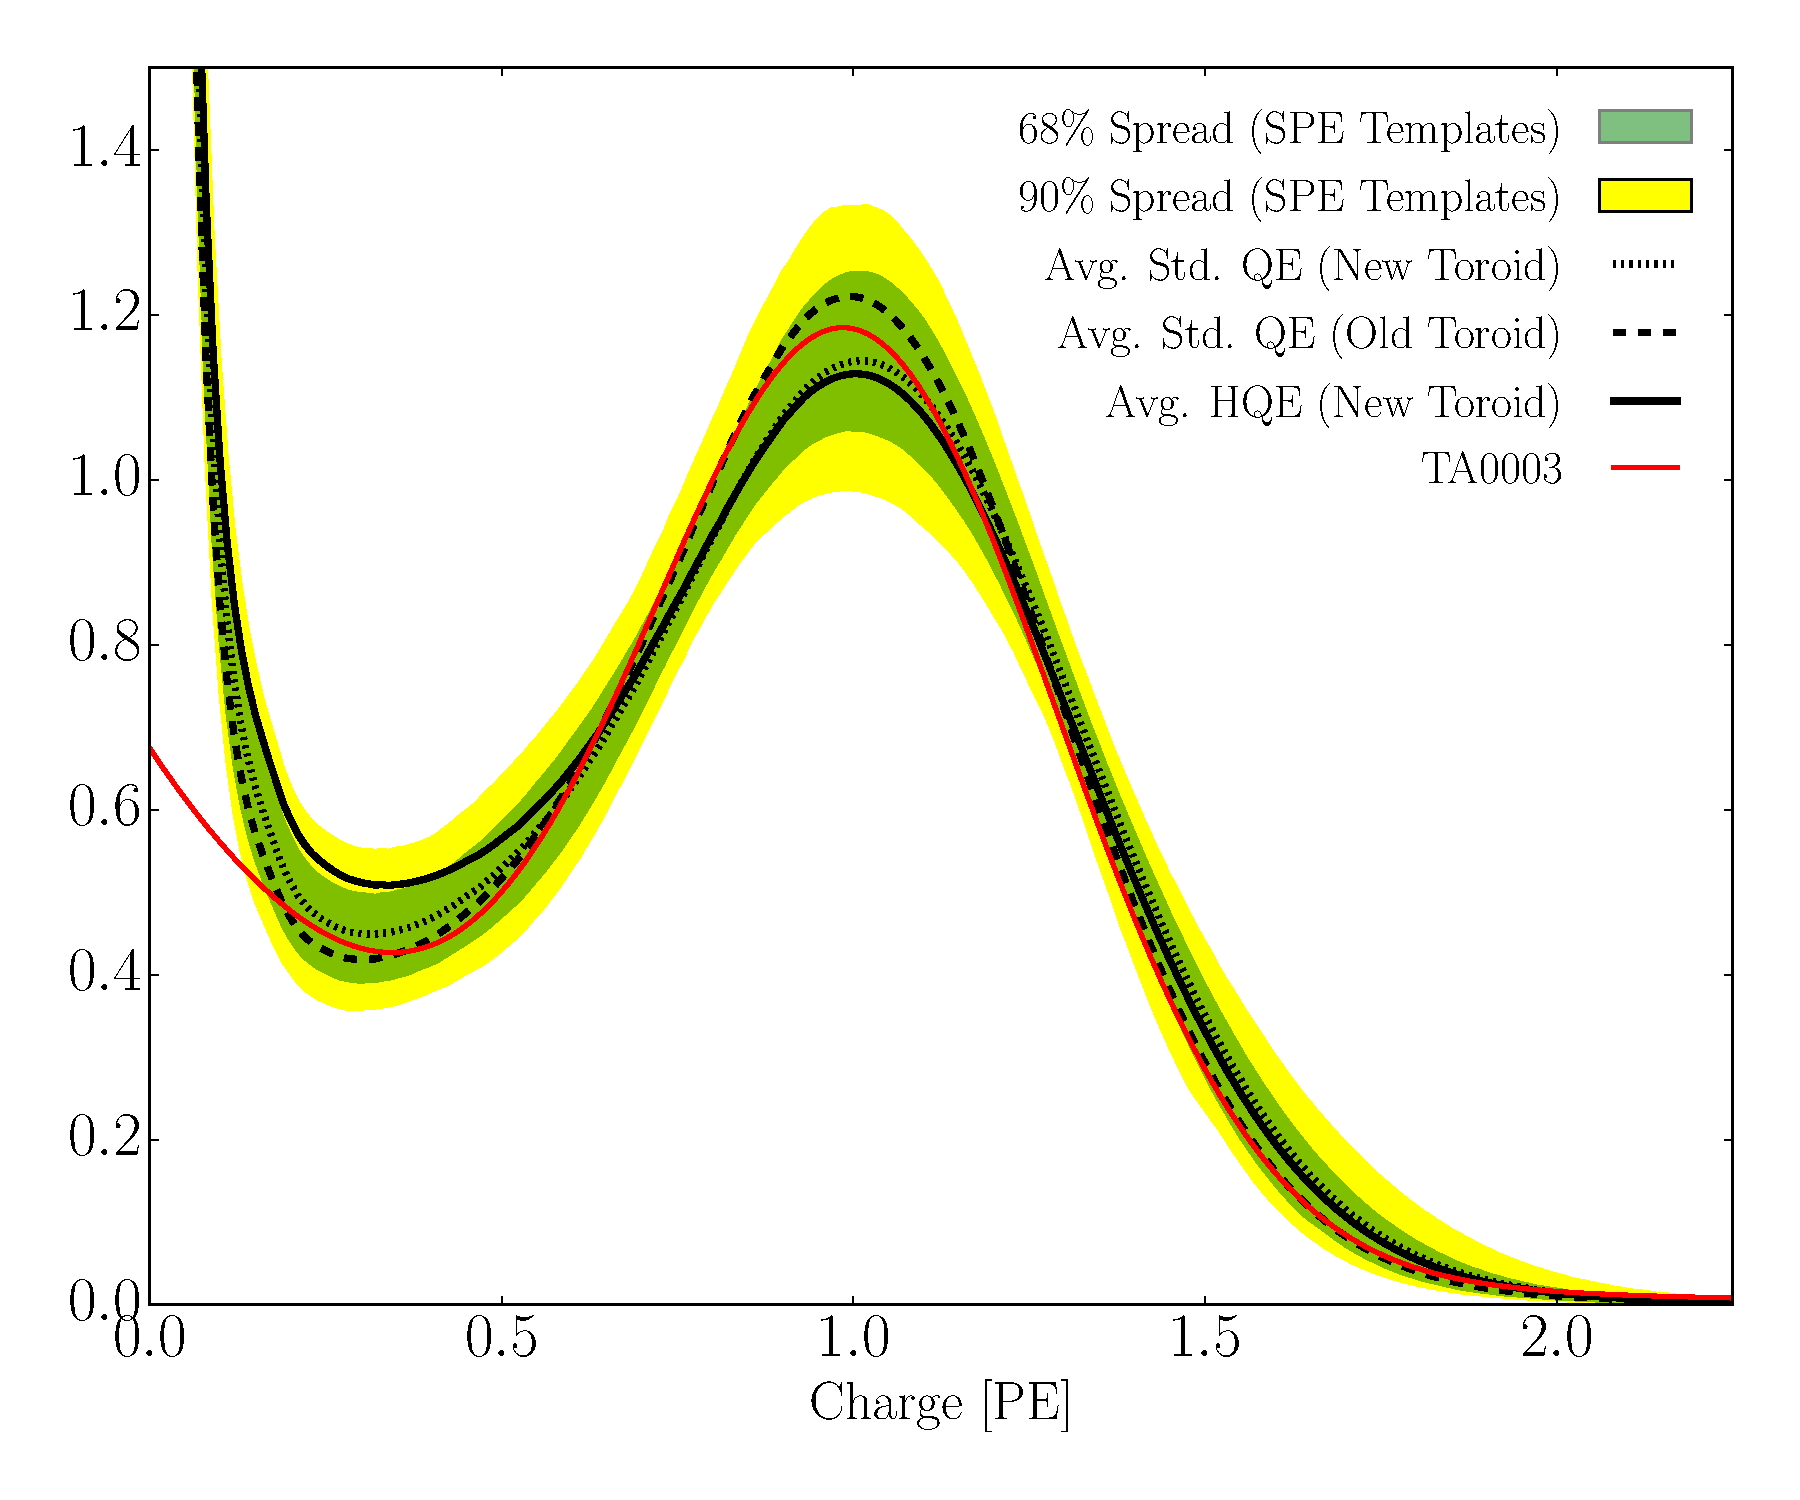
\includegraphics[width=.9\textwidth]{figures/simulation_and_processing/SPE_TA003_2.pdf}
	\caption[Single photo-electron charge distribution]{Single photo-electron charge distribution shown for a lab measurement in red (TA0003), various hardware configurations in black dashed, dotted, and solid lines, and the \SI{68}{\percent} and \SI{90}{\percent} spread of the measured charged templates for all DOMs. All curves are normalized to the same area. The figure is taken from \cite{spe_respose_pmt}.}
    \labfig{spe_distribution}
\end{figure}

Besides the Cherenkov photons, IceCube also observes photons that are produced in radioactive decays inside the DOMs, both in the glass housing sphere and the PMT glass itself. To simulate this internal noise, the \emph{Vuvuzela} module \sidecite{MLarson_master, MLarson_phd} is used to create additional MCPEs that are fed into the same simulation chain described above. The noise hits are simulated by drawing the times from a constant rate Poisson process and the number of photons from a Poisson distribution. Then the time differences between the individual photons per hit is found, based on a Log-Normal distribution. The simulation is defined by 5 parameters that are calibrated for each DOM individually. \reftab{vuvuzela_parameters} shows the average values for these parameters.
